\chapter{幻灯片制作}

2003年,柏林工业大学的博士生Till Tantau发布了一款用于制作演示文稿的工具Beamer。Beamer
是Till Tantau利用业余时间开发的,他的初衷是方便自己使用LaTeX制作幻灯片,不过出乎意料的是,
后来Beamer的受欢迎程度完全超出了他的想象。在Till Tantau开发Beamer期间,他收到了很多人的
建议和反馈,这些都直接推动了开发工作。2010年,Till Tantau将Beamer交由他人维护和管理。

Beamer作为LaTeX的一种特殊文档类型,它的出现无疑丰富了LaTeX制作演示文稿的功能。虽然Beamer
并非LaTeX中第一款用于制作演示文稿的工具,但直到今日,Beamer却是最受大家欢迎的一款。Beamer
的使用方式简单灵活,只需设定LaTeX文档类型为beamer,便可开始创作。同时,Beamer提供了大量
的幻灯片模板,这些模板包含了丰富多彩的视觉效果,创作者可以直接使用。毫不夸张地说,Beamer
的出现极大地提高了人们使用LaTeX制作幻灯片的热情。值得一提的是,在2005年,Till Tantau又
发布了一款非常便捷的LaTeX绘图工具TikZ。TikZ不仅可以辅助Beamer幻灯片的制作,也可以应用于
科技文档中的各类绘图任务。

Beamer是随着LaTeX的发展而衍生出来的一种特殊文档类型,也常常被看作是一个功能强大的宏包,
可以支撑科研工作者制作幻灯片的需求。使用Beamer制作幻灯片与Office办公软件(如PowerPoint)
完全不同,从本质上来说,使用Beamer制作幻灯片其实和LaTeX中的其他文档类型没有太大区别:
代码结构都是由前导代码和主体代码组成,完全沿用了LaTeX的文档环境与基本命令。因此,使用
Beamer制作幻灯片也有一个缺点,那就是必须掌握LaTeX制作文档的基础。

在呈现方式上,Beamer制作的幻灯片最终会在LaTeX中被编译成PDF文档,在不同的系统上打开幻灯
片时不存在不兼容等问题。在功能上,使用Beamer制作幻灯片时,我们可以对常规文本、公式、列
表、图表甚至动画效果、视觉效果和主题样式等进行调整,最终达到想要的视觉效果。

事实上,LaTeX中用于制作演示文稿的工具并非只有Beamer,但相比其他工具,Beamer具有如下优点:
\begin{itemize}
    \item 拥有海量的模板和丰富的主题样式,且使用方便;
    \item 能满足制作幻灯片的功能性需求,从创建标题、文本和段落到插入图表、参考文献等操作,且与常规文档中的使用规则几乎一致;
    \item 使用方式简单,在主体代码中使用frame环境就能创建一页幻灯片。
\end{itemize}

本章主要包括以下内容:Beamer的基本使用方式、在演示稿中添加动画效果、添加文本框等框元素、
设置主题样式、插入程序源代码、添加参考文献、插入表格、插入与调整图片。

\section{基本介绍}

Beamer是一款灵活的幻灯片制作工具,我们可以在LaTeX中将它作为一种文档类型进行使用。本节主
要介绍Beamer的基本使用方式,包括创建幻灯片、创建章节、生成目录等操作。

\subsection{Beamer简介}

在上述章节中,我们主要介绍了LaTeX中比较常用的文档类型article,可用于创建期刊论文、技术
报告等。本章中我们将介绍另一种文档类型:beamer。Beamer的开发者Till Tantau说,“BEAMER is a LATEX class for creating presentations”,显然,Beamer是一种用于制作演示文稿或者幻灯片的文档类型。

从使用角度来说,beamer文档类型和book、article等文档类型一样,都是在以\emph{.tex}为拓展名的文件
上编写程序和文档内容,然后再通过编译生成PDF文档。当然,Beamer也兼具常用演示文稿如PowerPoint
的主要功能,可以自行设置动态效果、甚至使用主题样式修改幻灯片的外观。

与其他文档类型相似的是,beamer文档类型中拥有很多视觉效果极好的模板,这些模版已经设置好了
特定的主题样式,有时候甚至只需要加入创作内容即可得到心仪的幻灯片。使用Beamer制作幻灯片时,
我们可以体验LaTeX排版论文的几乎所有优点,公式排版、图表排版、参考文献设置等也非常便捷,有
时候甚至可以将常规文档中的内容直接复制到Beamer文档类型中,稍加调整便能得到样式合适的幻灯
片。另外,我们也可以根据需要,在前导代码中使用全局设置调整幻灯片的主题样式、颜色主题、字体主题等。

使用beamer制作幻灯片仍然遵循着LaTeX的一般使用方法,代码结构分为前导代码和主体代码,前导
代码除了申明文档类型为beamer外,即\texttt{\textbackslash{}documentclass\{beamer\}},
调用宏包等与常规文档的制作基本是一致的。

\emph{【例】}使用beamer文档类型创建一个简单的幻灯片:
\begin{lstlisting}[language=TeX]
    \documentclass{beamer}

    \title{A Simple Beamer Example}
    \author{Author's Name}
    \institute{Author's Institute}
    \date{\today} 

    \begin{document}

    \frame{\titlepage}

    \end{document}
\end{lstlisting}

编译后得到的幻灯片如图\ref{fig:901}所示。

\begin{figure}[htbp]
    \centering
    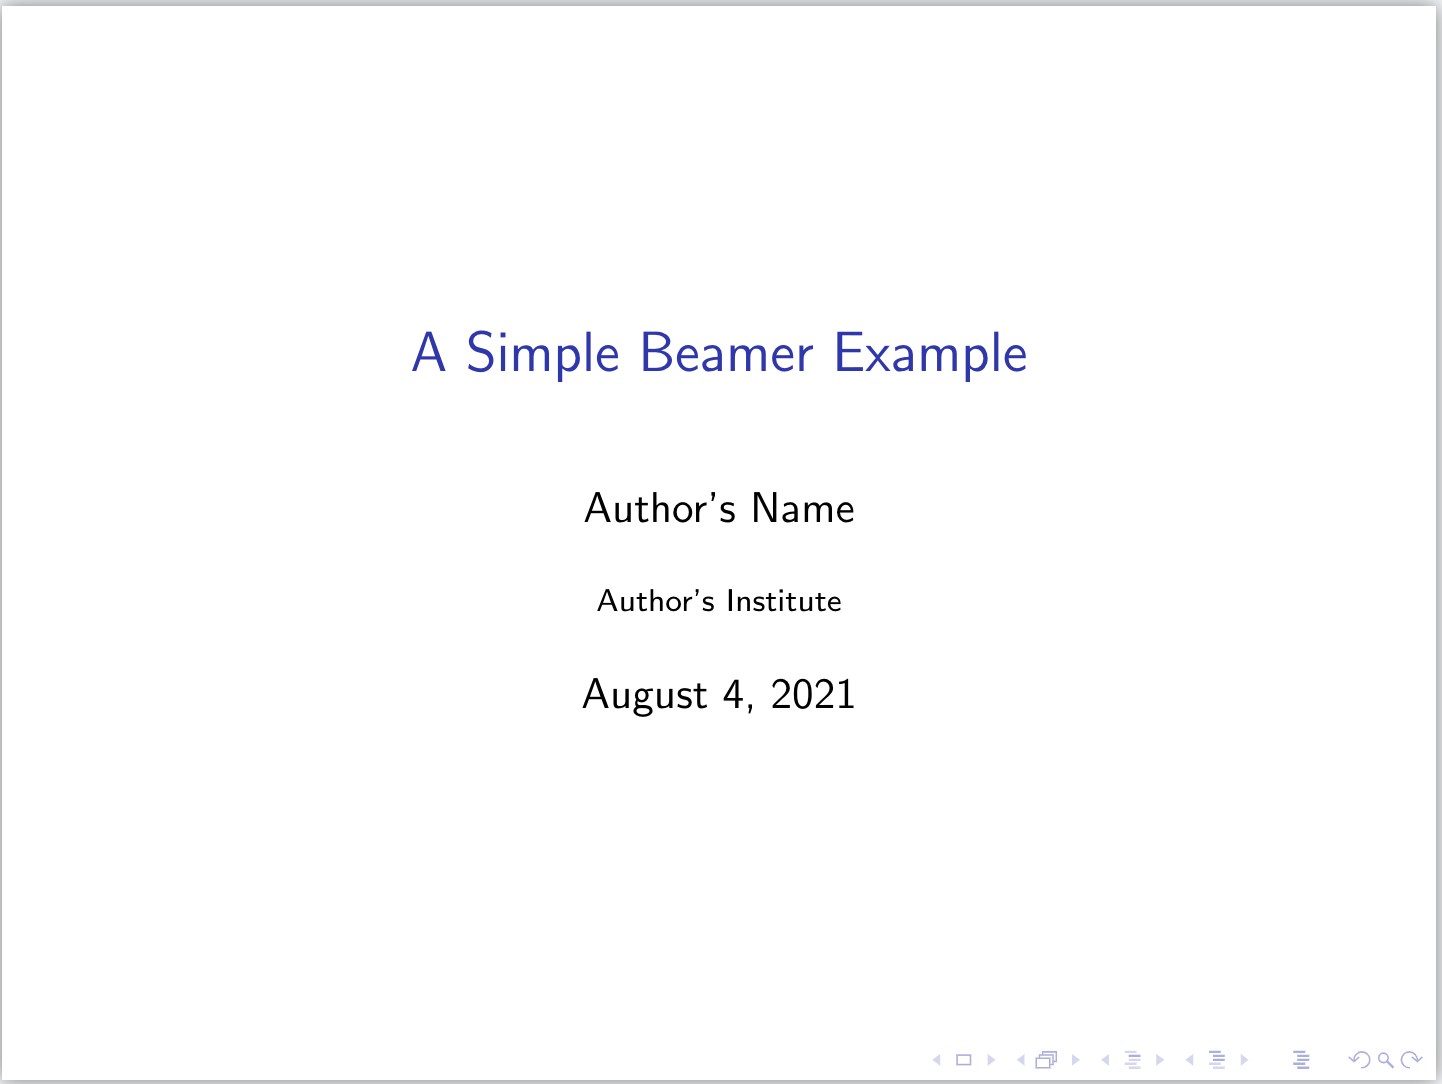
\includegraphics[width = 0.5\textwidth]{images/ch_9/example1.png}
    \caption{编译后的幻灯片效果}
    \label{fig:901}
\end{figure}


在例子中,\texttt{\textbackslash{}title\{\}}、\texttt{\textbackslash{}author\{\}}和
\texttt{\textbackslash{}date\{\}}这几个命令分别对应着标题、作者以及日期,一般放在标题
页,如果想在幻灯片首页显示这些信息,可以在使用\texttt{\textbackslash{}frame\{\textbackslash{}titlepage\}}
命令新建标题页。

总结来说,标题及作者信息对应的特定命令包括:
\begin{itemize}
    \item 标题:对应的命令为\texttt{\textbackslash{}title[A]\{B\}},其中,位置A一般填写的是简化标题,而位置B则填写的是完整标题,这里的完整标题有时候可能会很长。
    \item 副标题:对应的命令为\texttt{\textbackslash{}subtitle[A]\{B\}},其中,位置A一般填写的是简化副标题,而位置B则填写的是完整副标题,这里的完整副标题有时候也可能会很长。
    \item 作者:对应的命令为\texttt{\textbackslash{}author[A]\{B\}},用法类似。
    \item 日期:对应的命令为\texttt{\textbackslash{}date[A]\{B\}},用法类似。
    \item 单位:对应的命令为\texttt{\textbackslash{}institution[A]\{B\}},用法类似。
\end{itemize}

我们知道,在常规文档article中,申明文档类型时可以指定正文字体大小,在文档类型的申明语句
\texttt{\textbackslash{}documentclass\{beamer\}}中,我们也可以通过特定选项调整幻灯片
内容的字体大小,一般默认为11pt,我们也可以根据需要使用8pt、9pt、10pt、12pt、14pt、17pt、20pt
字体大小,例如使用\texttt{\textbackslash{}documentclass[12pt]\{beamer\}}可以将字体大小设置为12pt。

制作幻灯片时,有时候为了达到特定的投影效果,会设置幻灯片的长宽比例,比较常用的两种长宽比
例分别为4:3和16:9。一般来说,Beamer制作出来的幻灯片默认大小为长128毫米、宽96毫米,对应
着默认的长宽比例4:3,有时候,我们也可以根据需要将幻灯片的长宽比例调整为16:9、14:9、5:4
甚至3:2。

\emph{【例】}使用beamer文档类型创建一个简单的幻灯片,将幻灯片的长宽比例调整为16:9:
\begin{lstlisting}[language=TeX]
    \documentclass[aspectratio = 169]{beamer}

    \title{A Simple Beamer Example}
    \author{Author's Name}
    \institute{Author's Institute}
    \date{\today} 

    \begin{document}

    \frame{\titlepage}

    \end{document}
\end{lstlisting}

编译后得到的幻灯片如图\ref{fig:902}所示。

\begin{figure}[htbp]
    \centering
    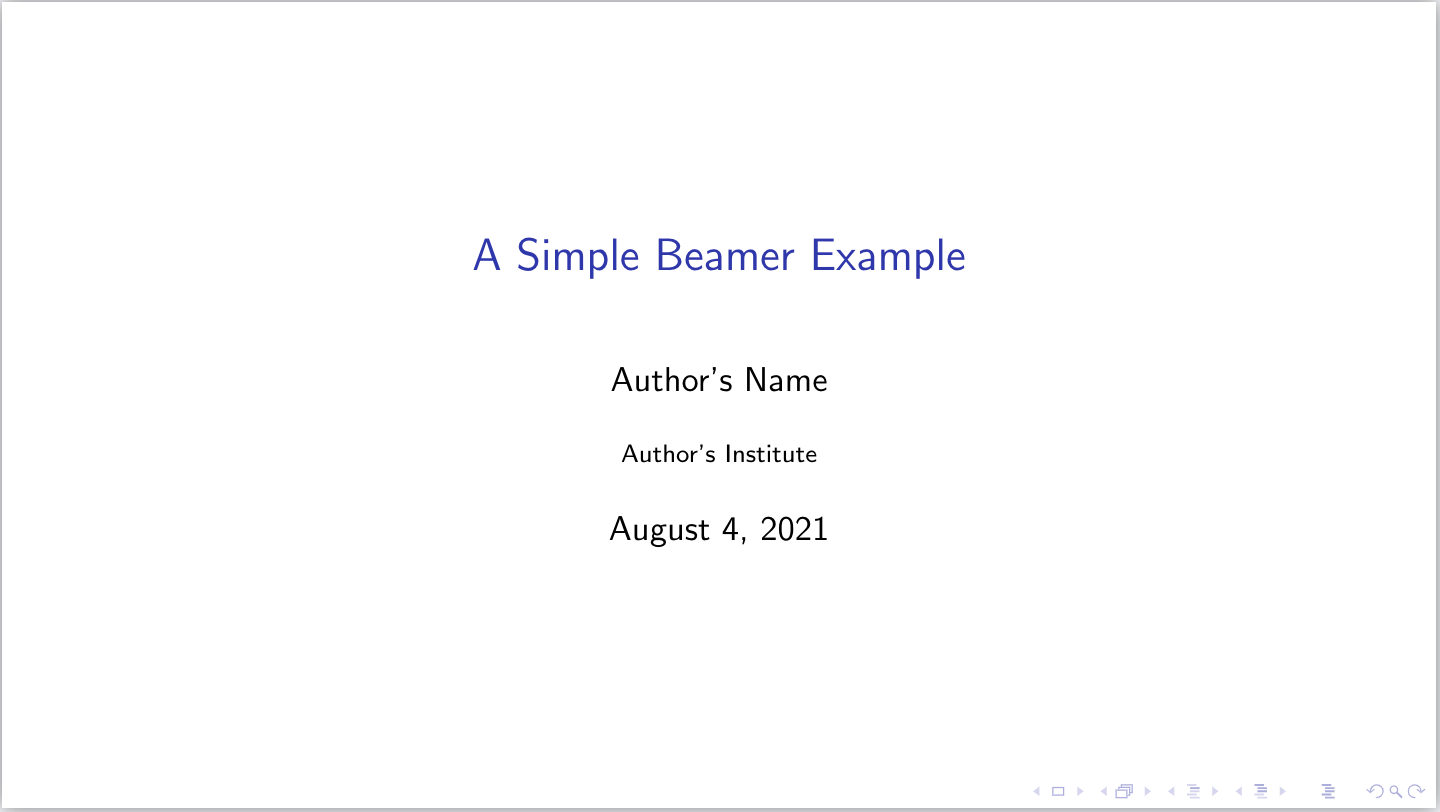
\includegraphics[width = 0.5\textwidth]{images/ch_9/example2.png}
    \caption{编译后的幻灯片效果}
    \label{fig:902}
\end{figure}


在例子中,选项aspectratio对应着长宽比例,数字169对应着长宽比例16:9,类似地,149、54、32
分别对应着长宽比例14:9、5:4、3:2。

\subsection{创建幻灯片}

frame这个词在计算机编程中非常常见,这一英文单词的字面意思可以翻译为“帧”,假如我们将幻灯
片视作“连环画”,是由一页一页单独的幻灯片组成,那么每一页幻灯片则对应着连环画中的帧。使用
Beamer制作幻灯片时,幻灯片就是用frame环境创建出来的,然而,有时候为了让幻灯片产生动画视
觉效果,Beamer中的帧(即frame)与每页幻灯片并非严格意义上的一一对应。

在beamer文档类型中,制作幻灯片的环境一般为frame。在document环境构成的主体代码中,一个frame
环境一般对应着一页幻灯片。

每张幻灯片一般都有一个标题,有时也会有一个副标题。若要创建标题和副标题,用户可以通过使用
\texttt{\textbackslash{}begin{frame}\{\}\{\}}的命令格式,其中第一、二个\{\}中分别为
幻灯片的标题和副标题;此外,用户也可以通过在frame环境中,使用\texttt{\textbackslash{}frametitle\{\}}
和\texttt{\textbackslash{}framesubtitle\{\}}命令分别创建标题和副标题。由此创建的标题
和副标题一般位于幻灯片的顶部,标题相对于副标题字体稍大一点。

实际上,Beamer与其他文档类型并没有特别大的差异,常规文档中的基本列表环境都可以在Beamer中
使用,包括:有序列表环境enumerate、无序列表环境itemize以及解释性列表环境description。

\emph{【例】}使用beamer文档类型创建一个简单的幻灯片:
\begin{lstlisting}[language=TeX]
    \documentclass{beamer}
    \usefonttheme{professionalfonts}

    \begin{document}

    \begin{frame}
    \frametitle{Parent function}
    \framesubtitle{A short list}

    Please check out the following parent function list.
    \begin{enumerate}
    \item $y=x$
    \item $y=|x|$
    \item $y=x^{2}$
    \item $y=x^{3}$
    \item $y=x^{b}$
    \end{enumerate}

    \end{frame}

    \end{document}
\end{lstlisting}

编译后得到的幻灯片如图\ref{fig:903}所示。

\begin{figure}[htbp]
    \centering
    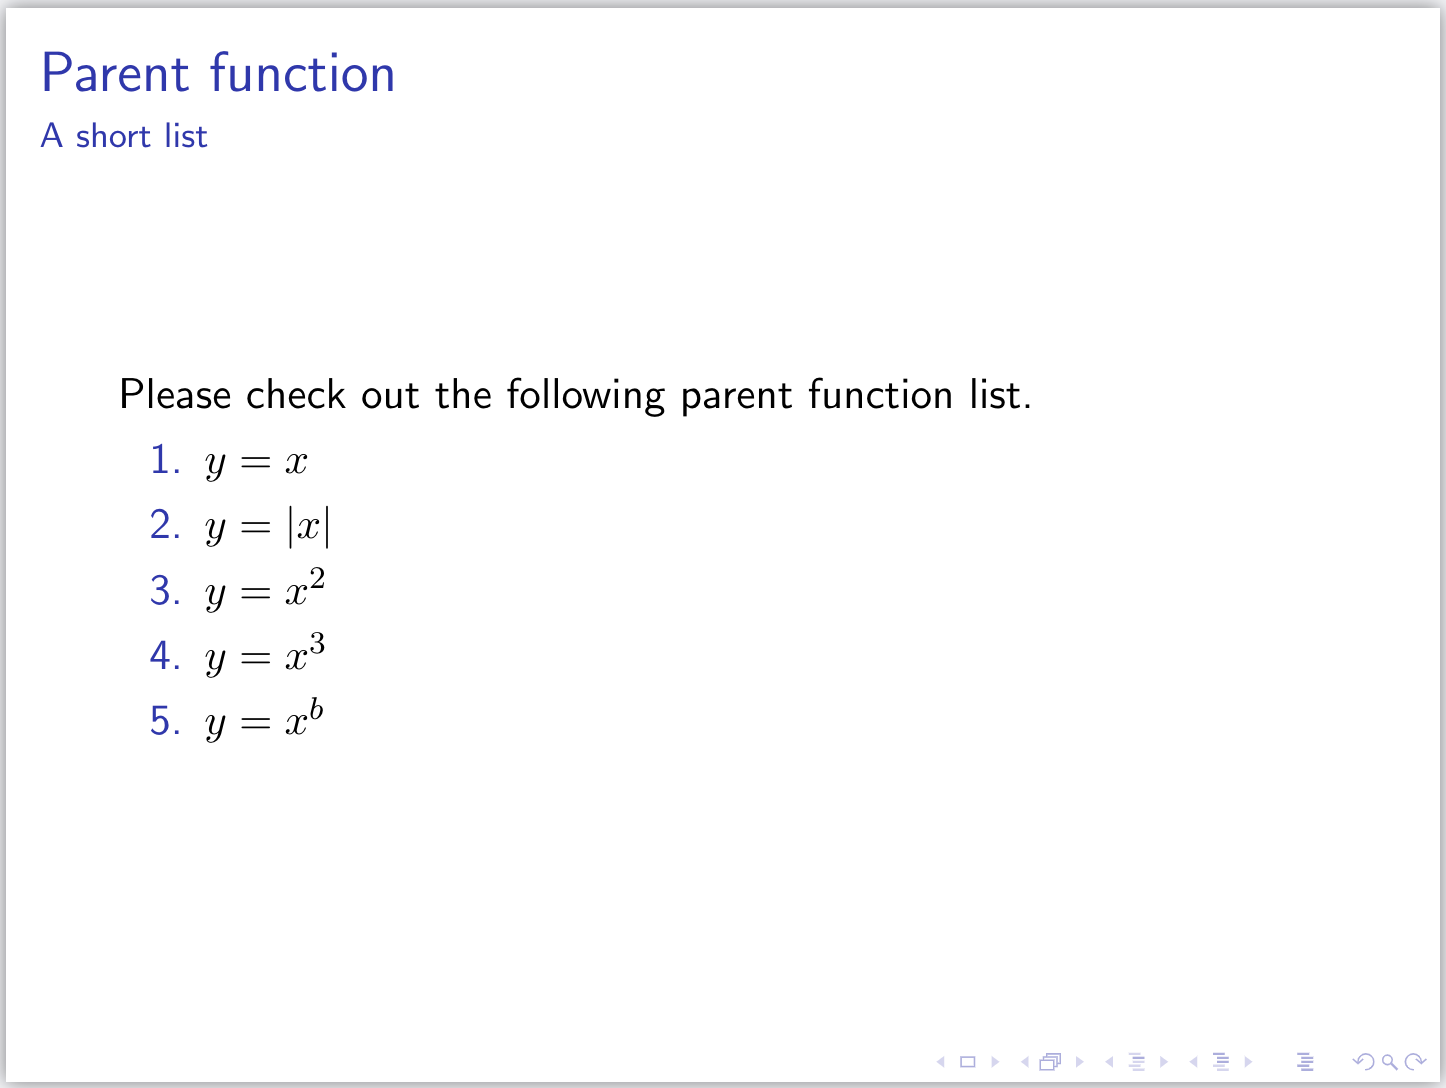
\includegraphics[width = 0.5\textwidth]{images/ch_9/example3.png}
    \caption{编译后的幻灯片效果}
    \label{fig:903}
\end{figure}

有时为了简化代码,也可以直接用\texttt{\textbackslash{}frame\{\}}命令取代frame环境囊括
幻灯片内容。

\emph{【例】}使用beamer文档类型中的frame简化环境命令创建一个简单的幻灯片:
\begin{lstlisting}[language=TeX]
    \documentclass{beamer}
    \usefonttheme{professionalfonts}

    \begin{document}

    \frame{
    \frametitle{Parent function}
    \framesubtitle{A short list}

    Please check out the following parent function list.
    \begin{enumerate}
    \item $y=x$
    \item $y=|x|$
    \item $y=x^{2}$
    \item $y=x^{3}$
    \item $y=x^{b}$
    \end{enumerate}

    \end{document}
\end{lstlisting}

使用Beamer制作幻灯片时,幻灯片内容会在标题下方自动居中对齐,如果想调整对其方式,可以在frame
环境中设置参数,具体而言,有以下几种:
\begin{itemize}
    \item [c] 居中对齐,字母c对应着英文单词center的首字母,一般而言,[c]作为默认参数,无需专门设置;
    \item [t] 让幻灯片内容进行顶部对齐,其中,字母t对应着英文单词top的首字母;
    \item [b] 让幻灯片内容进行底部对齐,其中,字母b对应着英文单词bottom的首字母。
\end{itemize}

\emph{【例】}使用beamer文档类型中的frame环境创建一个简单的幻灯片,并让幻灯片内容进行顶部对齐:
\begin{lstlisting}[language=TeX]
    \documentclass{beamer}
    \usefonttheme{professionalfonts}

    \begin{document}

    \begin{frame}[t]
    \frametitle{Parent function}
    \framesubtitle{A short list}

    Please check out the following parent function list.
    \begin{enumerate}
    \item $y=x$
    \item $y=|x|$
    \item $y=x^{2}$
    \item $y=x^{3}$
    \item $y=x^{b}$
    \end{enumerate}

    \end{frame}

    \end{document}
\end{lstlisting}

编译后得到的幻灯片如图\ref{fig:904}所示。

\begin{figure}[htbp]
    \centering
    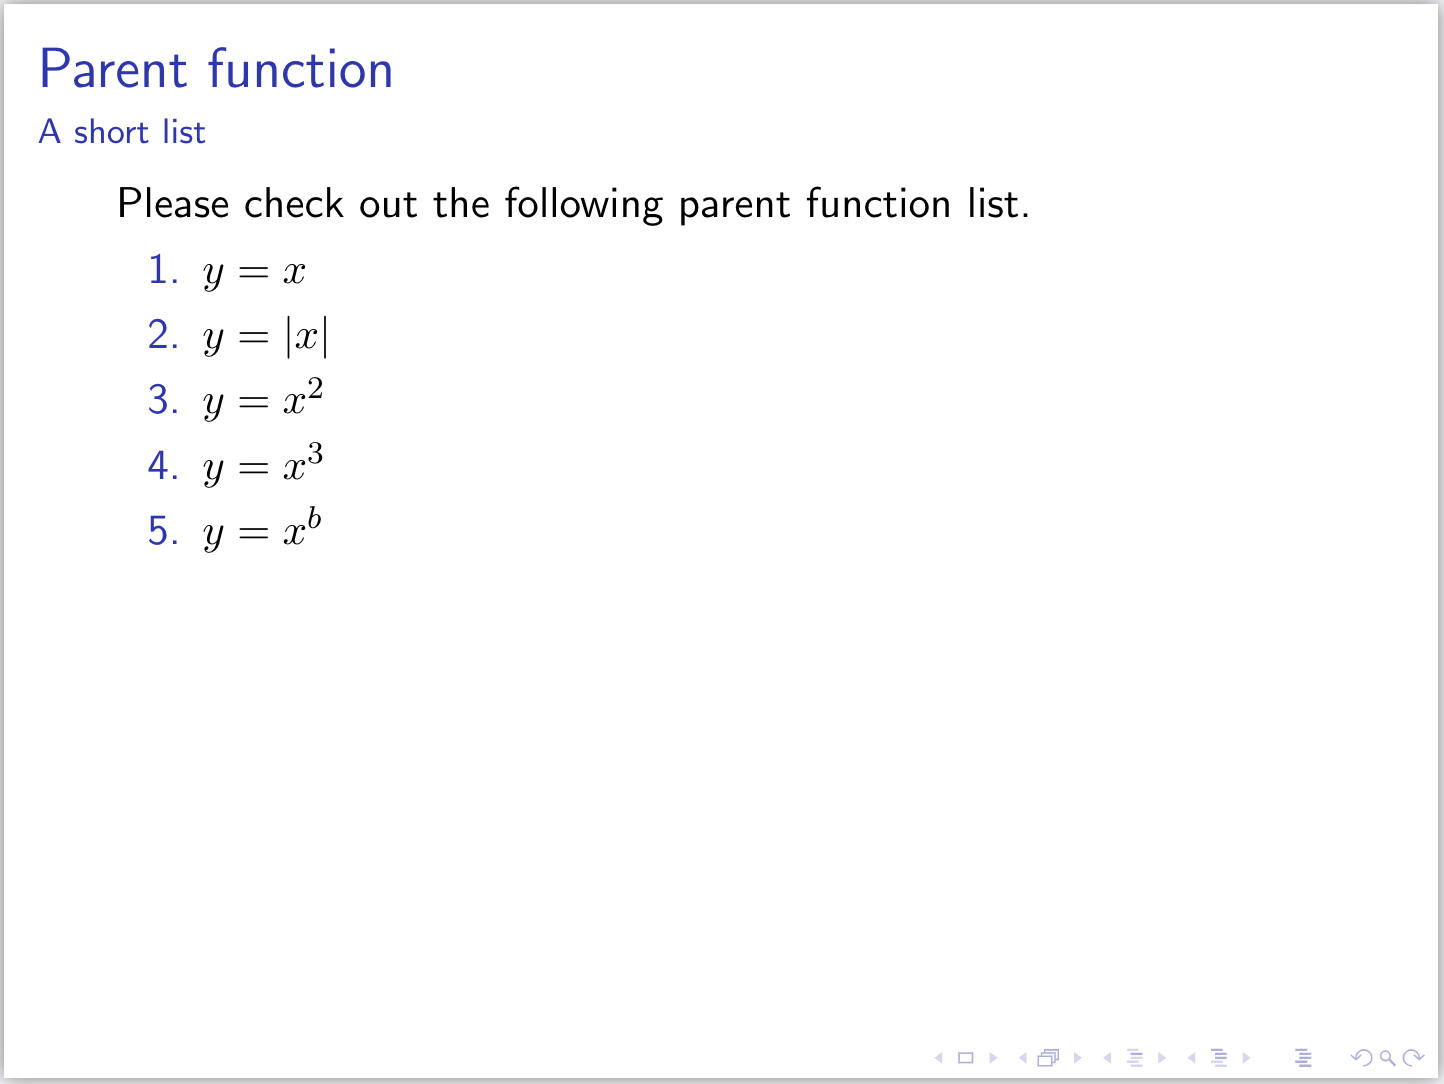
\includegraphics[width = 0.5\textwidth]{images/ch_9/example4.png}
    \caption{编译后的幻灯片效果}
    \label{fig:904}
\end{figure}

上面例子介绍了如何创建单页幻灯片,类似地,可以使用多个frame环境制作多页幻灯片。

\emph{【例】}使用beamer文档类型中的frame环境创建一个多页的幻灯片:
\begin{lstlisting}[language=TeX]
    \documentclass{beamer}

    \title{The title}
    \subtitle{The subtitle}
    \author{Author's name}

    \begin{document}

    \begin{frame}
        \titlepage % 创建标题页
    \end{frame}

    \begin{frame}
    \frametitle{Frame title}
    The body of the frame.
    \end{frame}

    \end{document}
\end{lstlisting}

编译后得到的幻灯片如图\ref{fig:905}所示。

\begin{figure}[htbp]
    \centering
    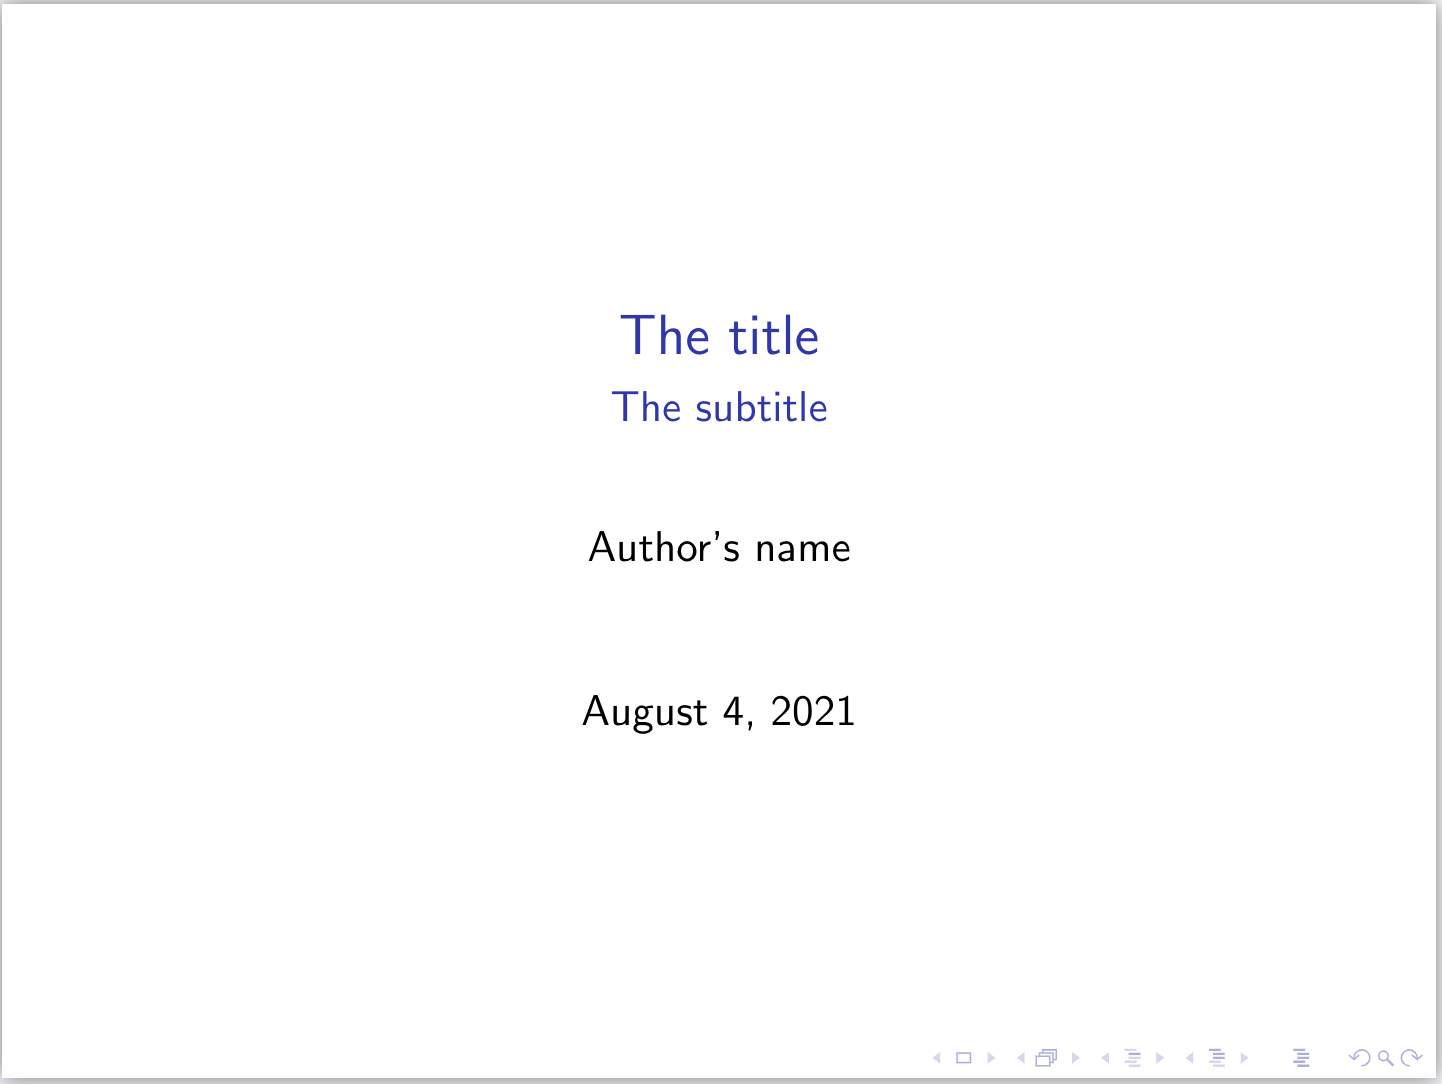
\includegraphics[width = 0.45\linewidth]{images/ch_9/example5_1.png}
    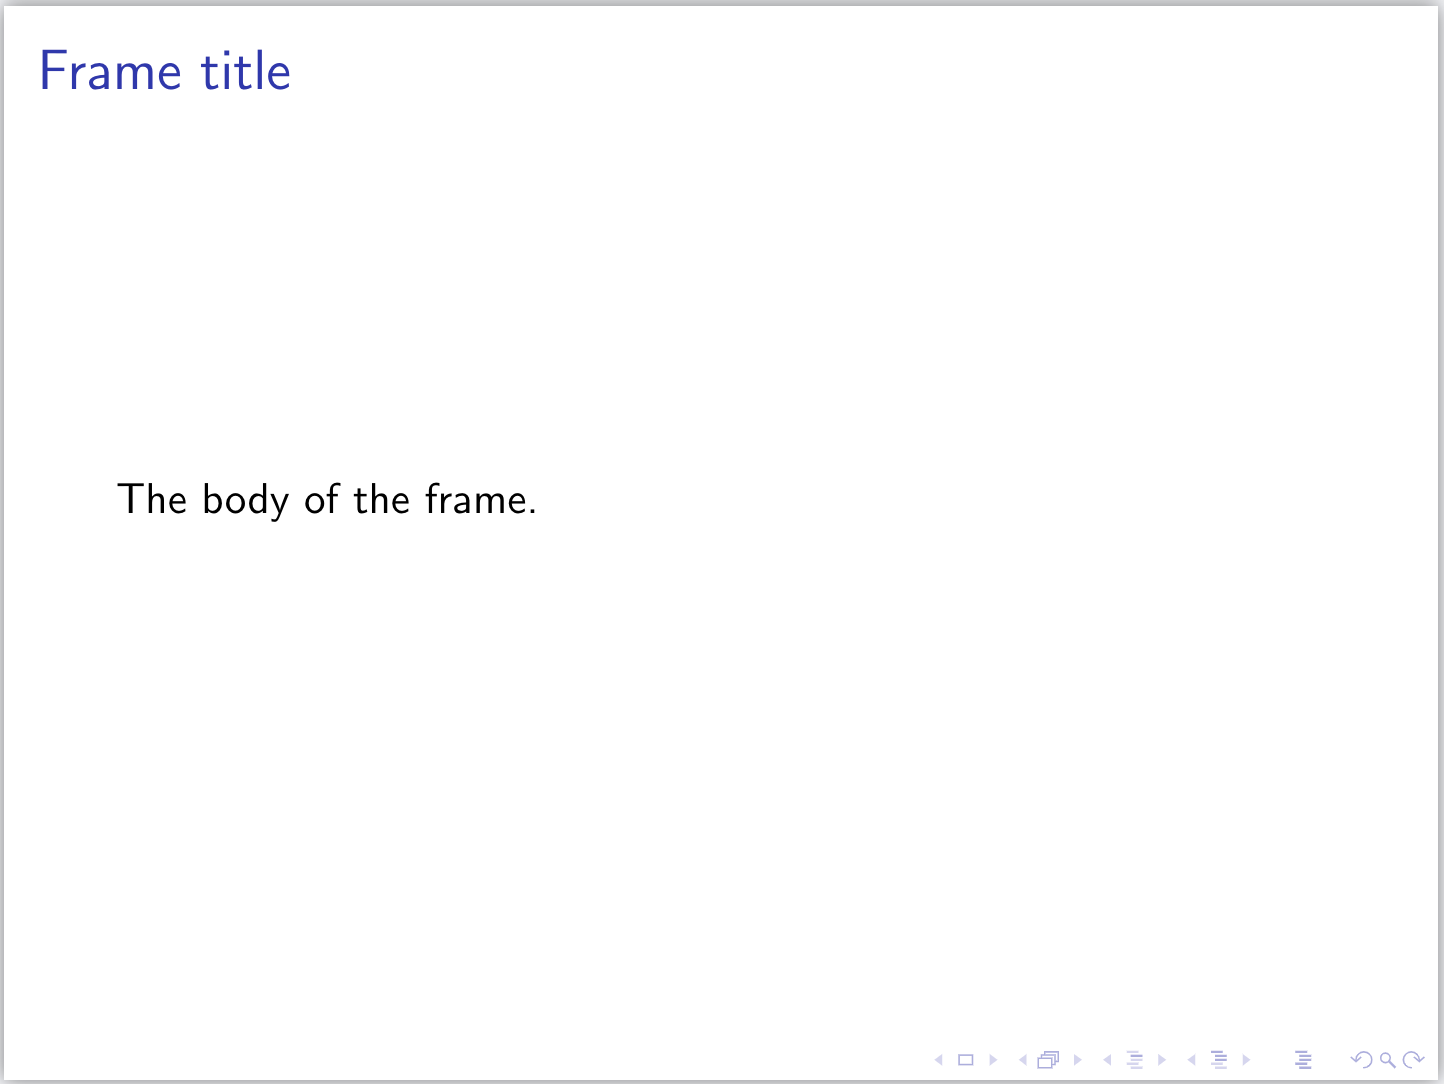
\includegraphics[width = 0.45\linewidth]{images/ch_9/example5_2.png}
    \caption{编译后的幻灯片效果}
    \label{fig:905}
\end{figure}

\subsection{创建章节与生成目录}

类似article文档类,beamer中可以利用\texttt{\textbackslash{}part\{\}}、\texttt{\textbackslash{}section\{\}}、
\texttt{\textbackslash{}subsection\{\}}、以及\texttt{\textbackslash{}subsubsection\{\}}等命令构建演示稿中的章节层次,但此时\texttt{\textbackslash{}chapter\{\}}命令无效。其中,章节标题写在\{\}中,但编译后不会出现在创建章节的位置,仅在目录和导航条中显示。类似地,可以通过加\emph{*}号使得章节标题不出现在目录中,但仍然会在导航条中显示。

在beamer中,可以使用\texttt{\textbackslash{}tableofcontents}命令自动生成演示稿目录,通过在frame幻灯片页中添加该命令即可。由此生成的目录实际上是超链接,点击之后会自动跳转到相应章节。

\emph{【例】}在beamer文档类型中使用tableofcontents命令为幻灯片生成目录,并使用section和subsection创建章节:
\begin{lstlisting}[language=TeX]
    \documentclass{beamer}

    \begin{document}

    \begin{frame}{Table of contents}
    \tableofcontents
    \end{frame}

    \section{Section A}
    \begin{frame}{frame1}
    \subsection{a1}
    This is subsection a1. This is subsection a1.
    \subsection{a2}
    This is subsection a2. This is subsection a2.
    \subsection{a3}
    This is subsection a3. This is subsection a3.
    \end{frame}

    \section{Section B}
    \begin{frame}{frame2}
    \subsection{b1}
    This is subsection b1. This is subsection b1. % 在下方插入空行,使得内容分行显示.

    \subsection{b2}
    This is subsection b2. % 在下方插入空行,使得内容分行显示.

    This is subsection b2.
    \end{frame}

    \section*{Section C}
    \begin{frame}{frame3}
    \subsection*{c1}
    This is subsection c1. This is subsection c1. % 在下方插入空行,使得内容分行显示.

    \subsection*{c2}
    This is subsection c2. This is subsection c2.
    \end{frame}

    \end{document}
\end{lstlisting}

编译后得到的幻灯片如图\ref{fig:906}所示。

\begin{figure}[htbp]
    \centering
    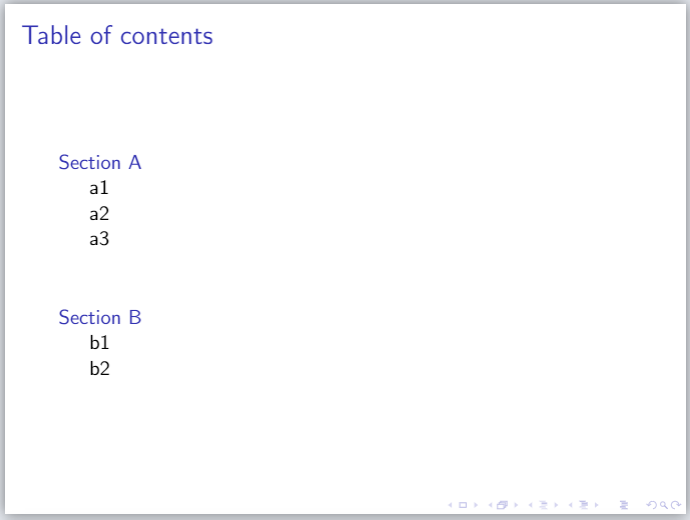
\includegraphics[width = 0.45\linewidth]{images/ch_9/example10NEW_1.png}
    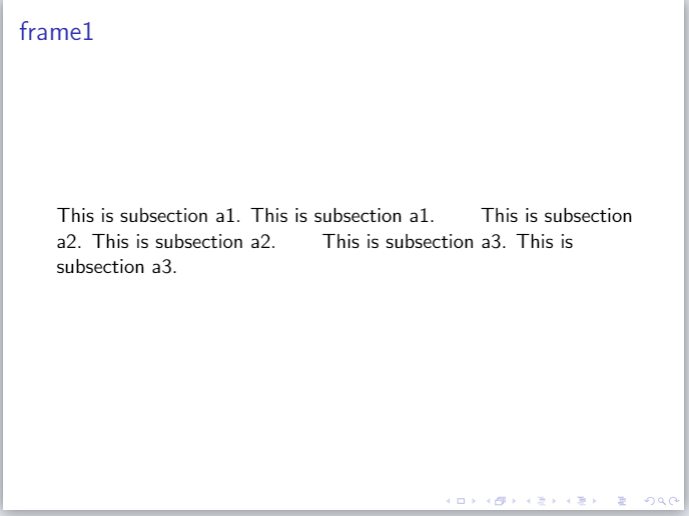
\includegraphics[width = 0.45\linewidth]{images/ch_9/example10NEW_2.png}
    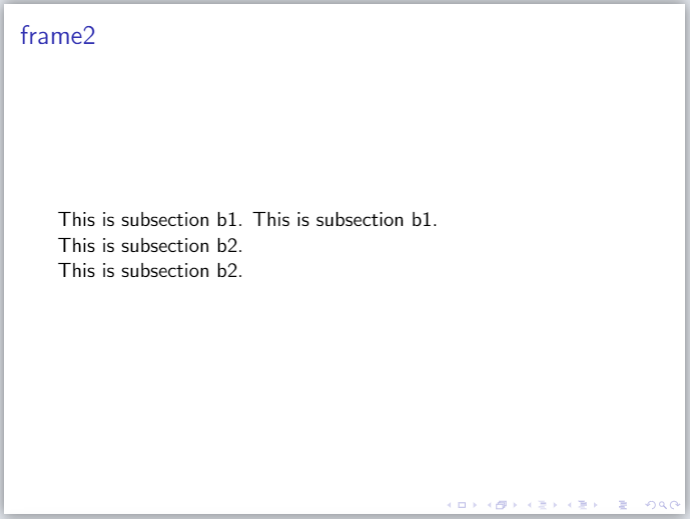
\includegraphics[width = 0.45\linewidth]{images/ch_9/example10NEW_3.png}
    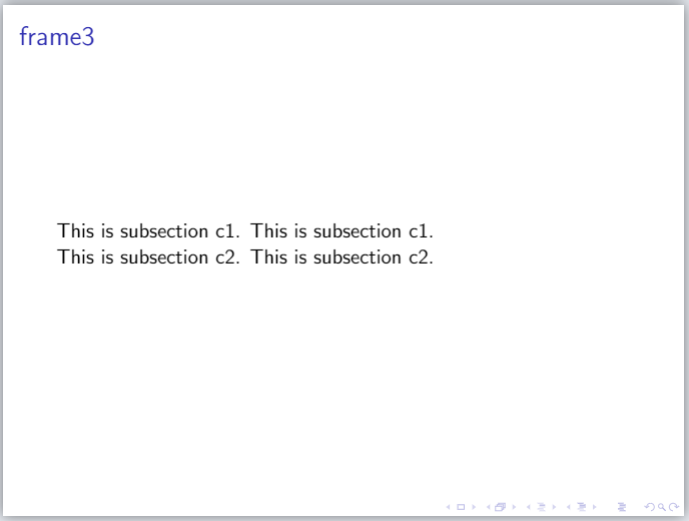
\includegraphics[width = 0.45\linewidth]{images/ch_9/example10NEW_4.png}
    \caption{编译后的幻灯片效果}
    \label{fig:906}
\end{figure}

从上例中可以看出,如果想让相邻章节或者同章节的内容分行显示,只需要在相应位置插入空行即可。

默认情况下,目录页中包含所有不含*号的章节标题,甚至是三级节标题。但有时目录只需要显示到一级节标题即可,而二级节标题及其次级标题则不需要显示,为此,只需要在\texttt{\textbackslash{}tableofcontents}命令后设置选项[hideallsubsections]即可。

\emph{【例】}在beamer文档类型中使用\texttt{\textbackslash{}tableofcontents[hideallsubsections]}命令为幻灯片生成一级节目录:
\begin{lstlisting}[language=TeX]
    \documentclass{beamer}

    \begin{document}

    \begin{frame}{table of contents}
    \tableofcontents[hideallsubsections]
    \end{frame}

    \section{Section A}
    \begin{frame}{frame1}
    \subsection{a1}
    This is subsection a1. This is subsection a1.

    \subsection{a2}
    This is subsection a2. This is subsection a2.

    \subsection{a3}
    This is subsection a3. This is subsection a3.

    \end{frame}

    \section{Section B}
    \begin{frame}{frame2}
    \subsection{b1}
    This is subsection b1. This is subsection b1.

    \subsection{b2}
    This is subsection b2. This is subsection b2.
    \end{frame}

    \end{document}
\end{lstlisting}

编译后得到的幻灯片如图\ref{fig:907}所示。

\begin{figure}[htbp]
    \centering
    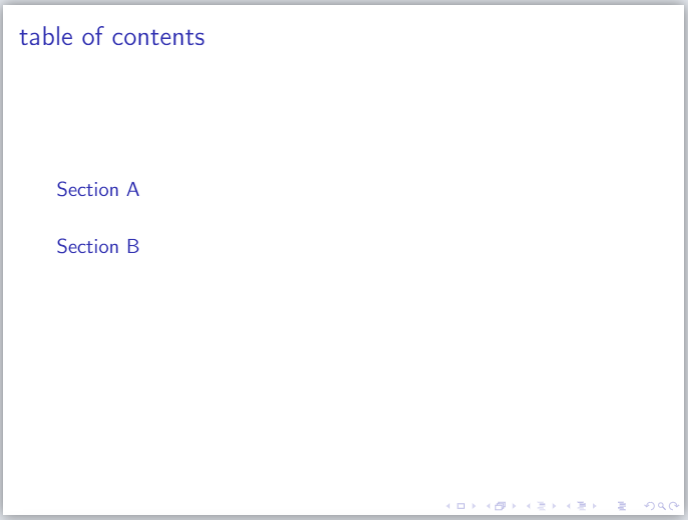
\includegraphics[width = 0.45\linewidth]{images/ch_9/NEWexample13_1.png}
    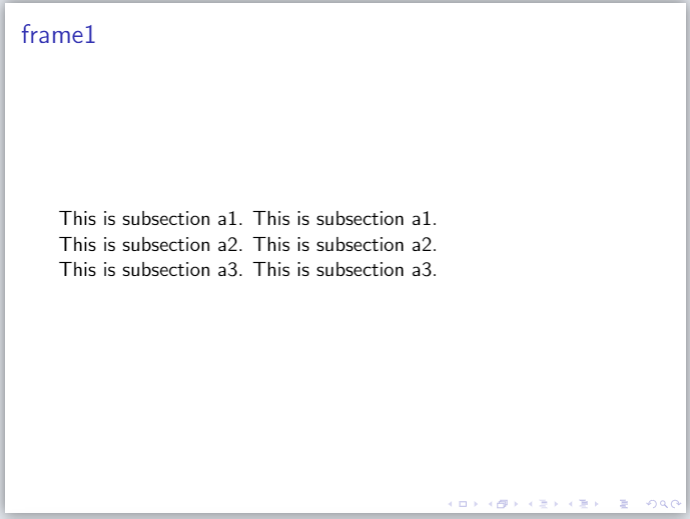
\includegraphics[width = 0.45\linewidth]{images/ch_9/NEWexample13_2.png}
    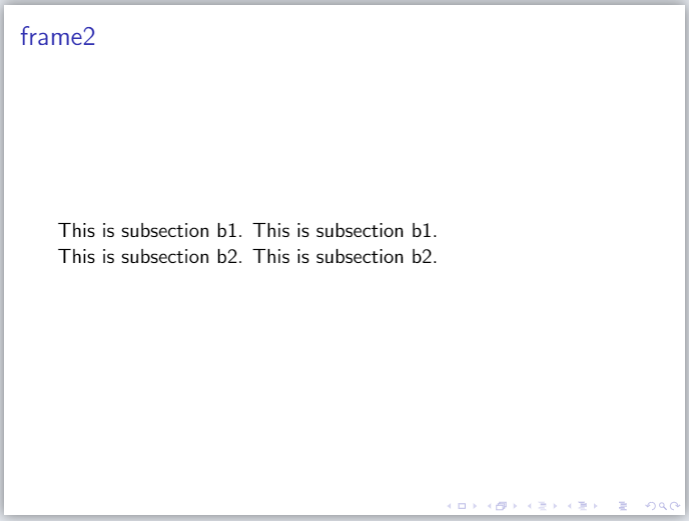
\includegraphics[width = 0.45\linewidth]{images/ch_9/NEWexample13_3.png}
    \caption{编译后的幻灯片效果}
    \label{fig:907}
\end{figure}

一般而言,使用\texttt{\textbackslash{}tableofcontents}命令生成的目录只会显示在相应的幻灯片页。有时候为了更好地梳理演示稿脉络,需要在各章节前均插入目录页,为此,一种更简便的方式是使用\texttt{\textbackslash{}AtBeginSection\{\}}、\texttt{\textbackslash{}AtBeginSubsection\{\}}、或\texttt{\textbackslash{}AtBeginSubsubsection\{\}}命令分别在一级节、二级节、三级节前均插入目录页。此外,使用\texttt{\textbackslash{}tableofcontents[currentsection]}命令或\texttt{\textbackslash{}tableofcontents[currentsubsection]}命令可以在各章节前的目录页中突出显示当前一级节标题或二级节标题。

\emph{【例】}在beamer文档类型中使用\texttt{\textbackslash{}AtBeginSection\{\}}以及\texttt{\textbackslash{}tableofcontents[currentsection]}命令在幻灯片的各一级节前均插入目录页,并突出显示当前一级节标题:
\begin{lstlisting}[language=TeX]
    \documentclass{beamer}

    \begin{document}

    \AtBeginSection
    {
    \begin{frame}{table of contents}
    \tableofcontents[currentsection]
    \end{frame}
    }

    \section{Section A}
    \begin{frame}{frame1}
    \subsection{a1}
    This is subsection a1. This is subsection a1.

    \subsection{a2}
    This is subsection a2. This is subsection a2.

    \subsection{a3}
    This is subsection a3. This is subsection a3.
    \end{frame}

    \section{Section B}
    \begin{frame}{frame2}
    \subsection{b1}
    This is subsection b1. This is subsection b1.

    \subsection{b2}
    This is subsection b2. This is subsection b2.
    \end{frame}

    \section{Section C}
    \begin{frame}{frame3}
    \subsection{c1}
    This is subsection c1. This is subsection c1.

    \subsection{c2}
    This is subsection c2. This is subsection c2.
    \end{frame}

    \end{document}
\end{lstlisting}

编译后得到的幻灯片如图\ref{fig:908}所示。

\begin{figure}[htbp]
    \centering
    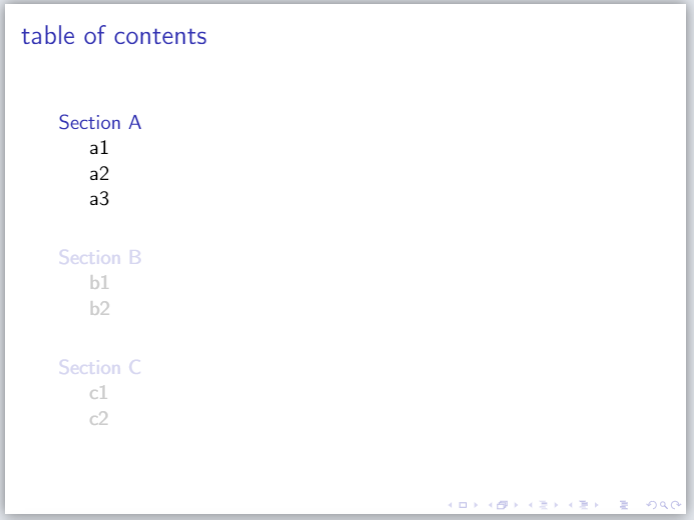
\includegraphics[width = 0.45\linewidth]{images/ch_9/NEWexample12_1.png}
    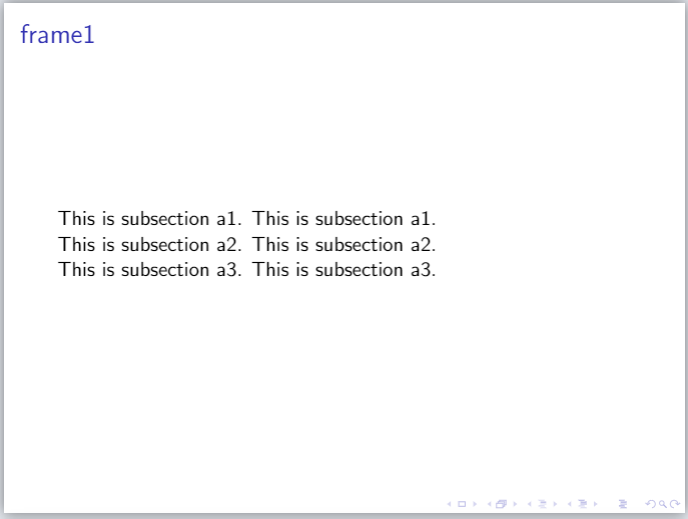
\includegraphics[width = 0.45\linewidth]{images/ch_9/NEWexample12_2.png}
    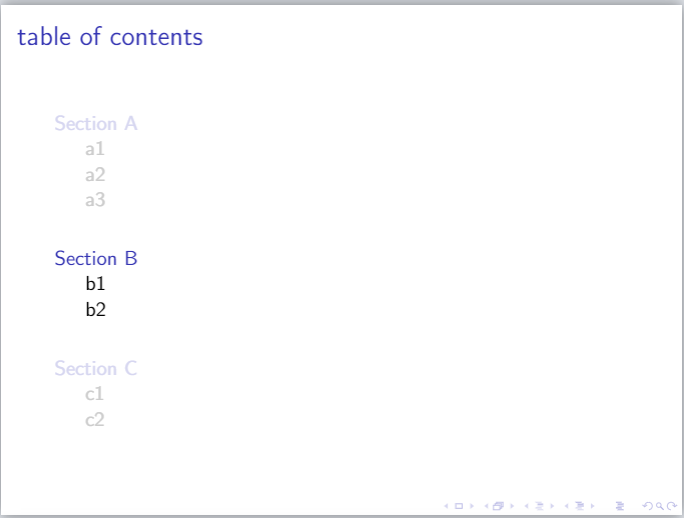
\includegraphics[width = 0.45\linewidth]{images/ch_9/NEWexample12_3.png}
    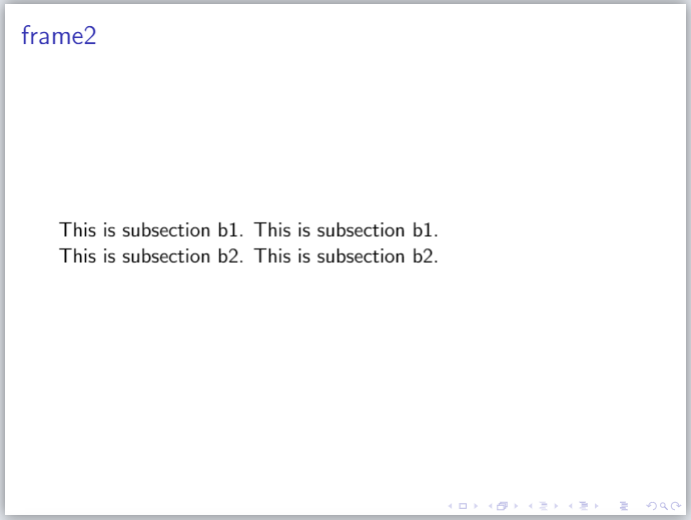
\includegraphics[width = 0.45\linewidth]{images/ch_9/NEWexample12_4.png}
    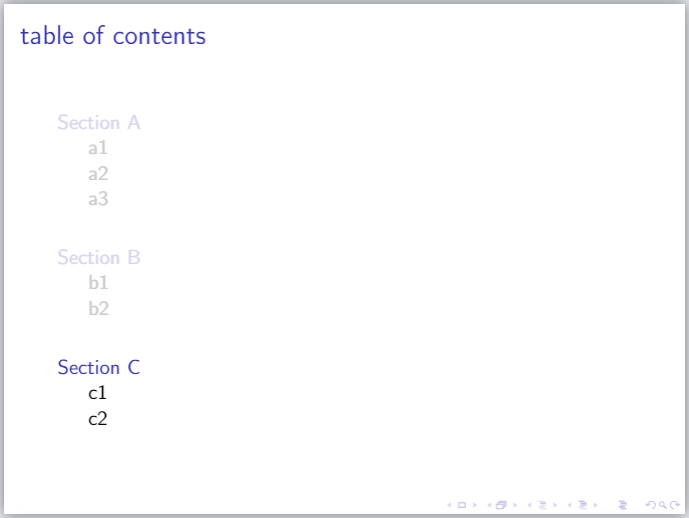
\includegraphics[width = 0.45\linewidth]{images/ch_9/NEWexample12_5.png}
    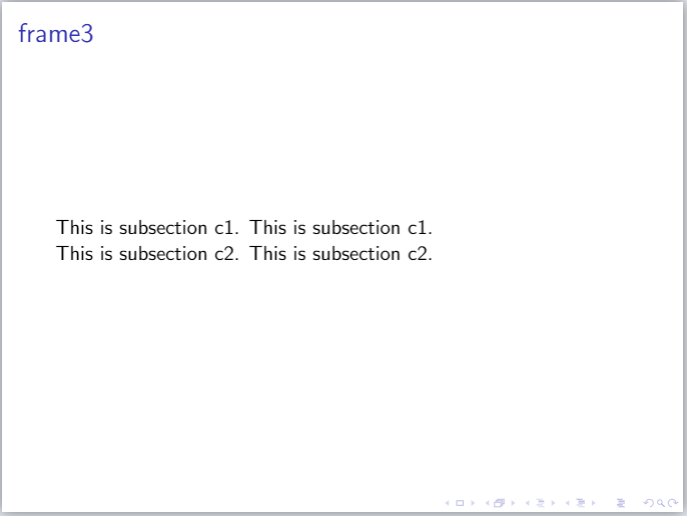
\includegraphics[width = 0.45\linewidth]{images/ch_9/NEWexample12_6.png}
    \caption{编译后的幻灯片效果}
    \label{fig:908}
\end{figure}

生成目录时,我们也能自定义目录显示的动画格式,通过使用\texttt{\textbackslash{}tableofcontents[pausesections]}命令,同时在前导代码中申明\texttt{\textbackslash{}setbeamercovered\{dynamic\}}语句即可。

\emph{【例】}在beamer文档类型中使用\texttt{\textbackslash{}tableofcontents}命令生成幻灯片的目录,同时使用\texttt{\textbackslash{}tableofcontents[pausesections]}对目录设置动画格式:
\begin{lstlisting}[language=TeX]
    \documentclass{beamer}
    \setbeamercovered{dynamic}

    \begin{document}

    \begin{frame}
    \frametitle{Table of Contents}

    \tableofcontents[pausesections]

    \end{frame}

    \section{Intro to Beamer}
    \subsection{About Beamer}
    \subsection[Basic Structure]{Basic Structure}
    \subsection{How to Compile}
    \section{Overlaying Concepts}
    \subsection{Specifications}
    \subsection[Examples]{Examples: Lists, Graphics, Tables}
    \section[Sparkle]{Adding that Sparkle}
    \subsection{Sections}
    \subsection{Themes}
    \section*{References}

    \begin{frame}

    \end{frame}

    \end{document}
\end{lstlisting}

编译后得到的幻灯片如图\ref{fig:909}所示。

\begin{figure}[htbp]
    \centering
    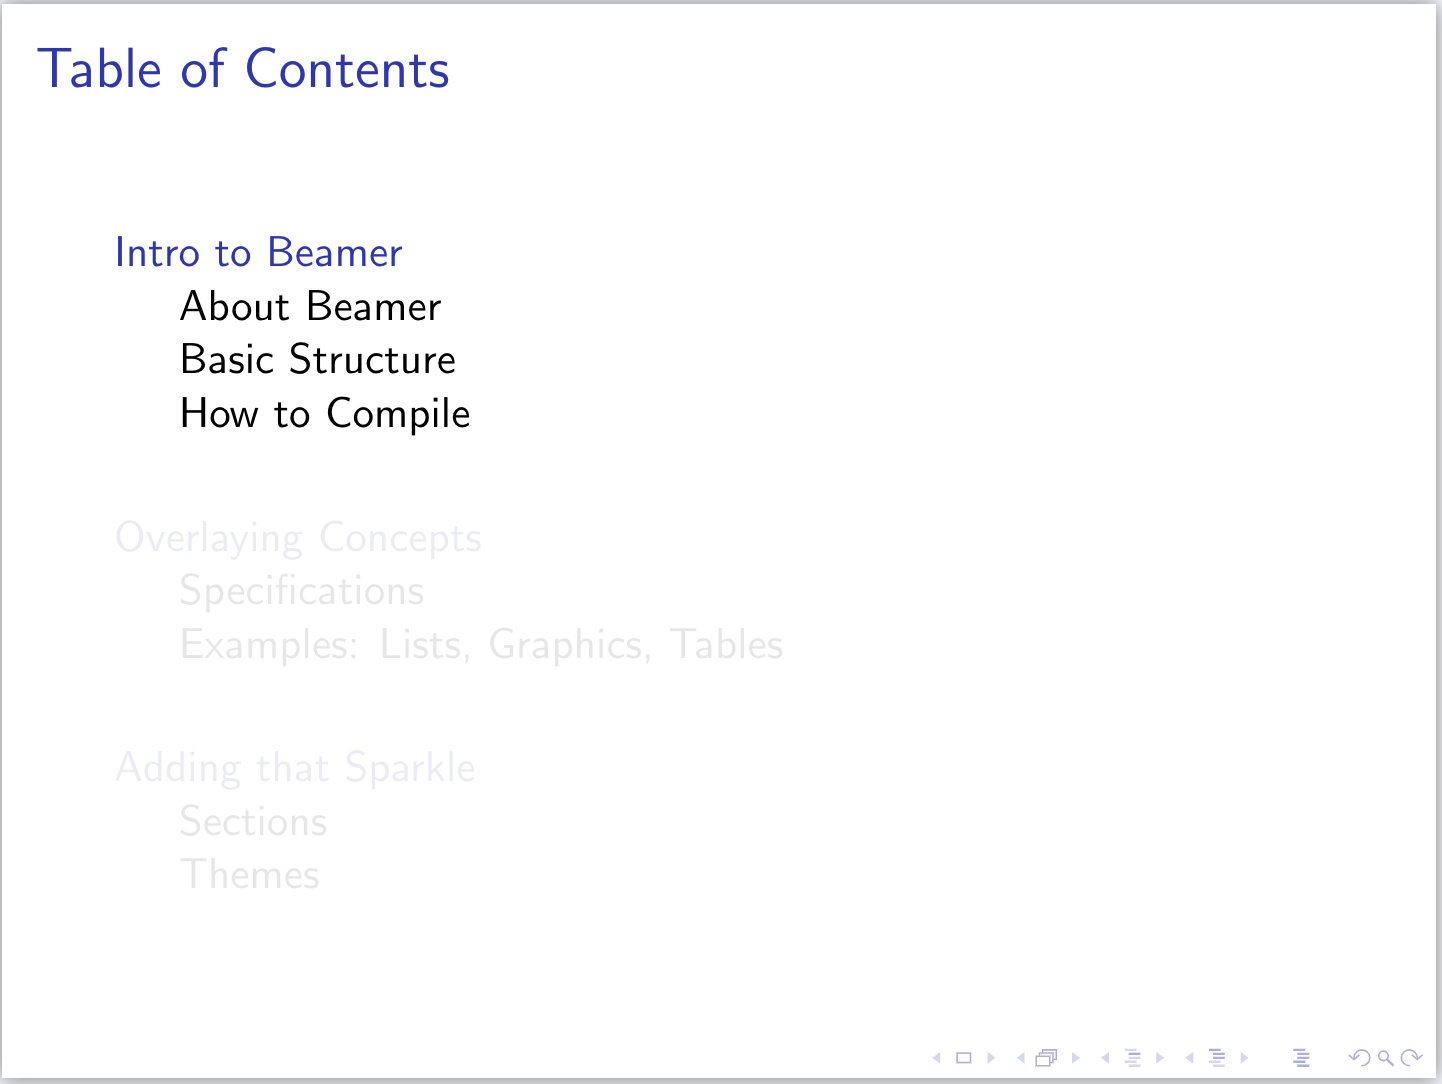
\includegraphics[width = 0.45\linewidth]{images/ch_9/example11_1.png}
    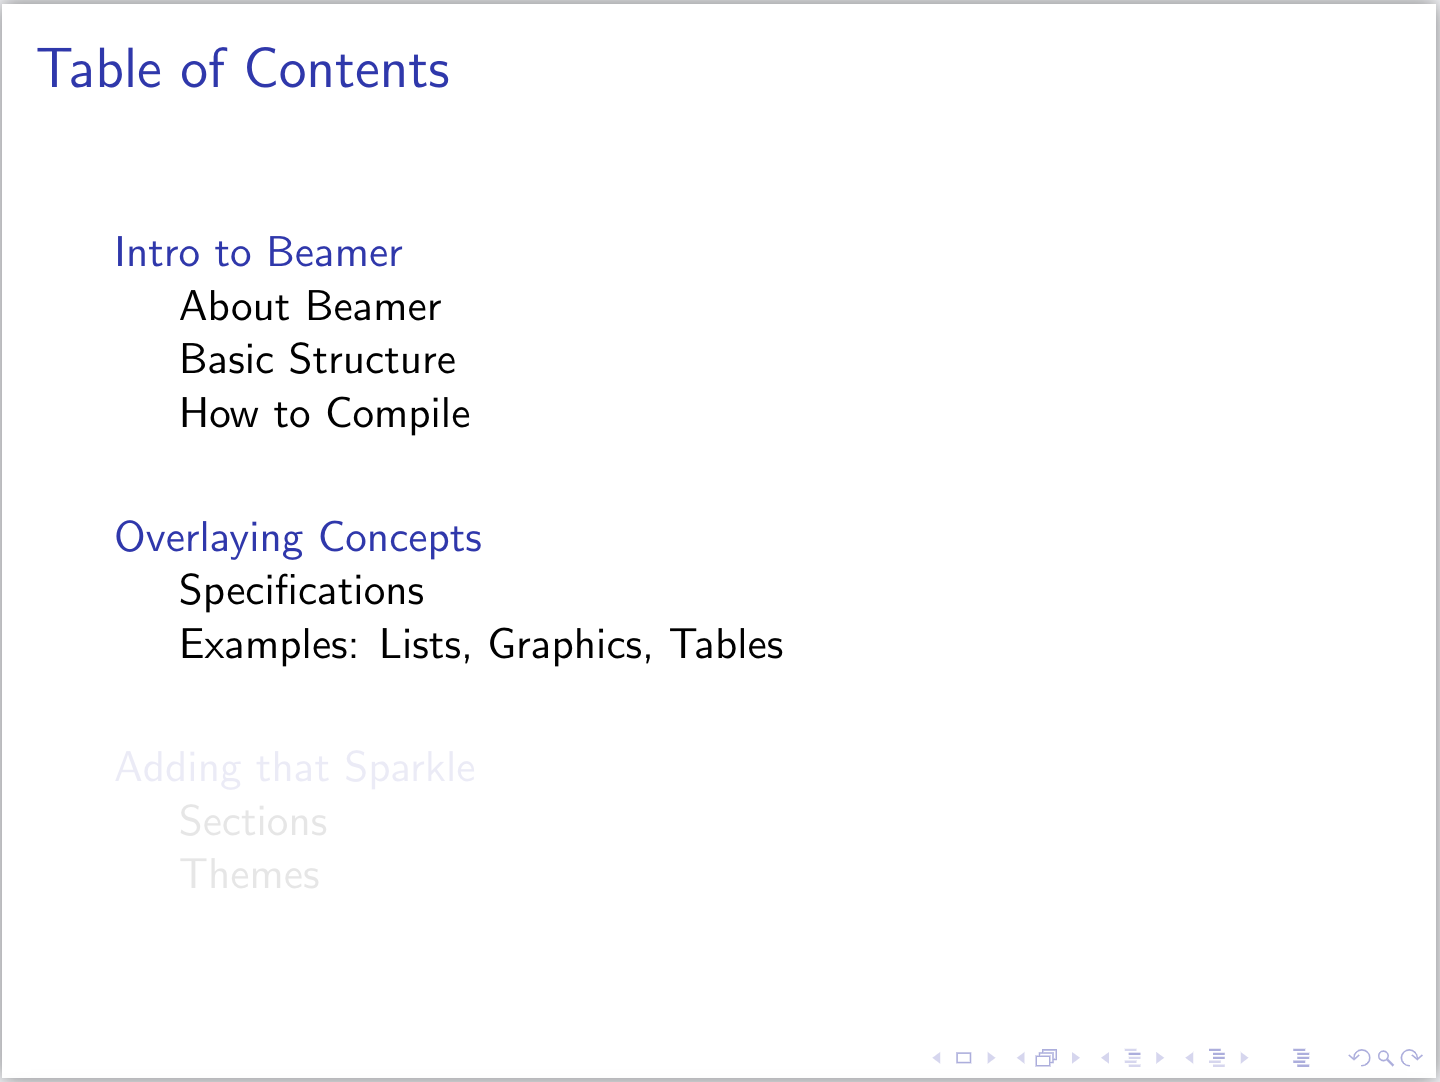
\includegraphics[width = 0.45\linewidth]{images/ch_9/example11_2.png}
    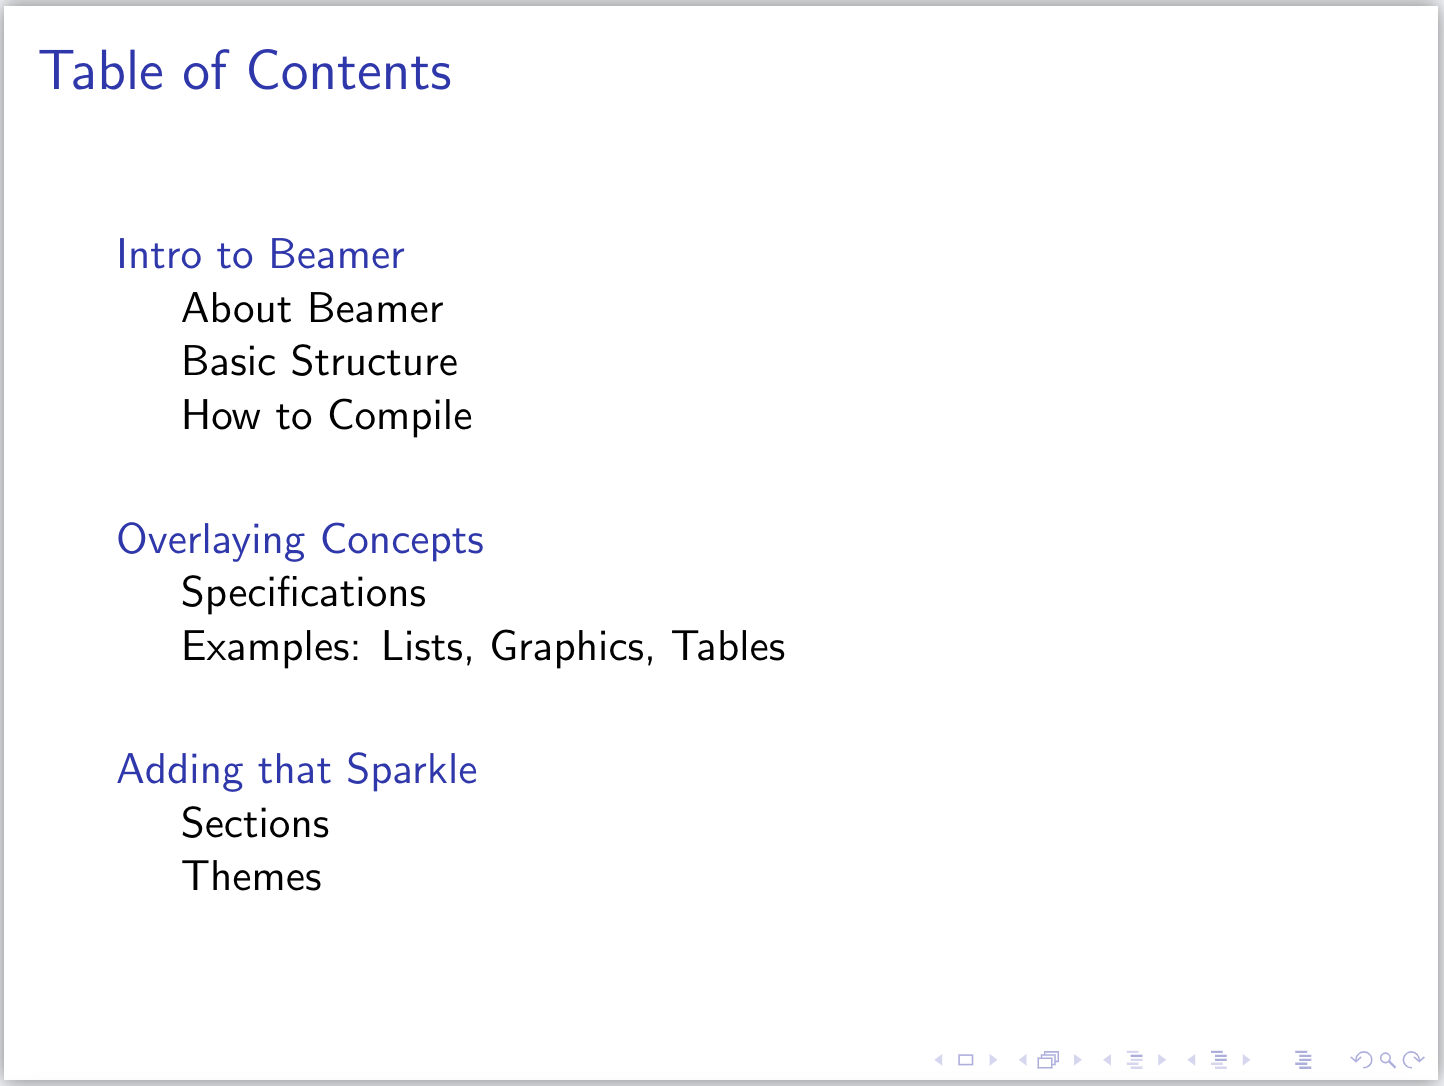
\includegraphics[width = 0.45\linewidth]{images/ch_9/example11_3.png}
    \caption{编译后的幻灯片效果}
    \label{fig:909}
\end{figure}

\subsection{幻灯片内容分栏}

对幻灯片内容进行分栏有两种常用方式,第一种是使用multicol宏包中的\text{\textbackslash{}begin\{multicols\}\{A\}} \texttt{\textbackslash{}end\{multicols\}}环境,其中位置A可用于设定分栏列数;第二种是使用\texttt{\textbackslash{}begin\{columns\}} \texttt{\textbackslash{}end\{columns\}}环境。

\emph{【例】}在beamer文档类型中使用multicol宏包对列表内容进行分栏处理:
\begin{lstlisting}[language=TeX]
    \documentclass{beamer}
    \usefonttheme{professionalfonts}
    \usepackage{multicol}

    \begin{document}

    \begin{frame}
    \frametitle{Parent function}
    \framesubtitle{A short list}

    Please check out the following parent function list.
    \begin{enumerate}
    \begin{multicols}{3}
    \item $y=x$
    \item $y=|x|$
    \item $y=x^{2}$
    \item $y=x^{3}$
    \item $y=x^{b}$
    \end{multicols}
    \end{enumerate}

    \end{frame}

    \end{document}
\end{lstlisting}

编译后得到的幻灯片如图\ref{fig:910}所示。

\begin{figure}[htbp]
    \centering
    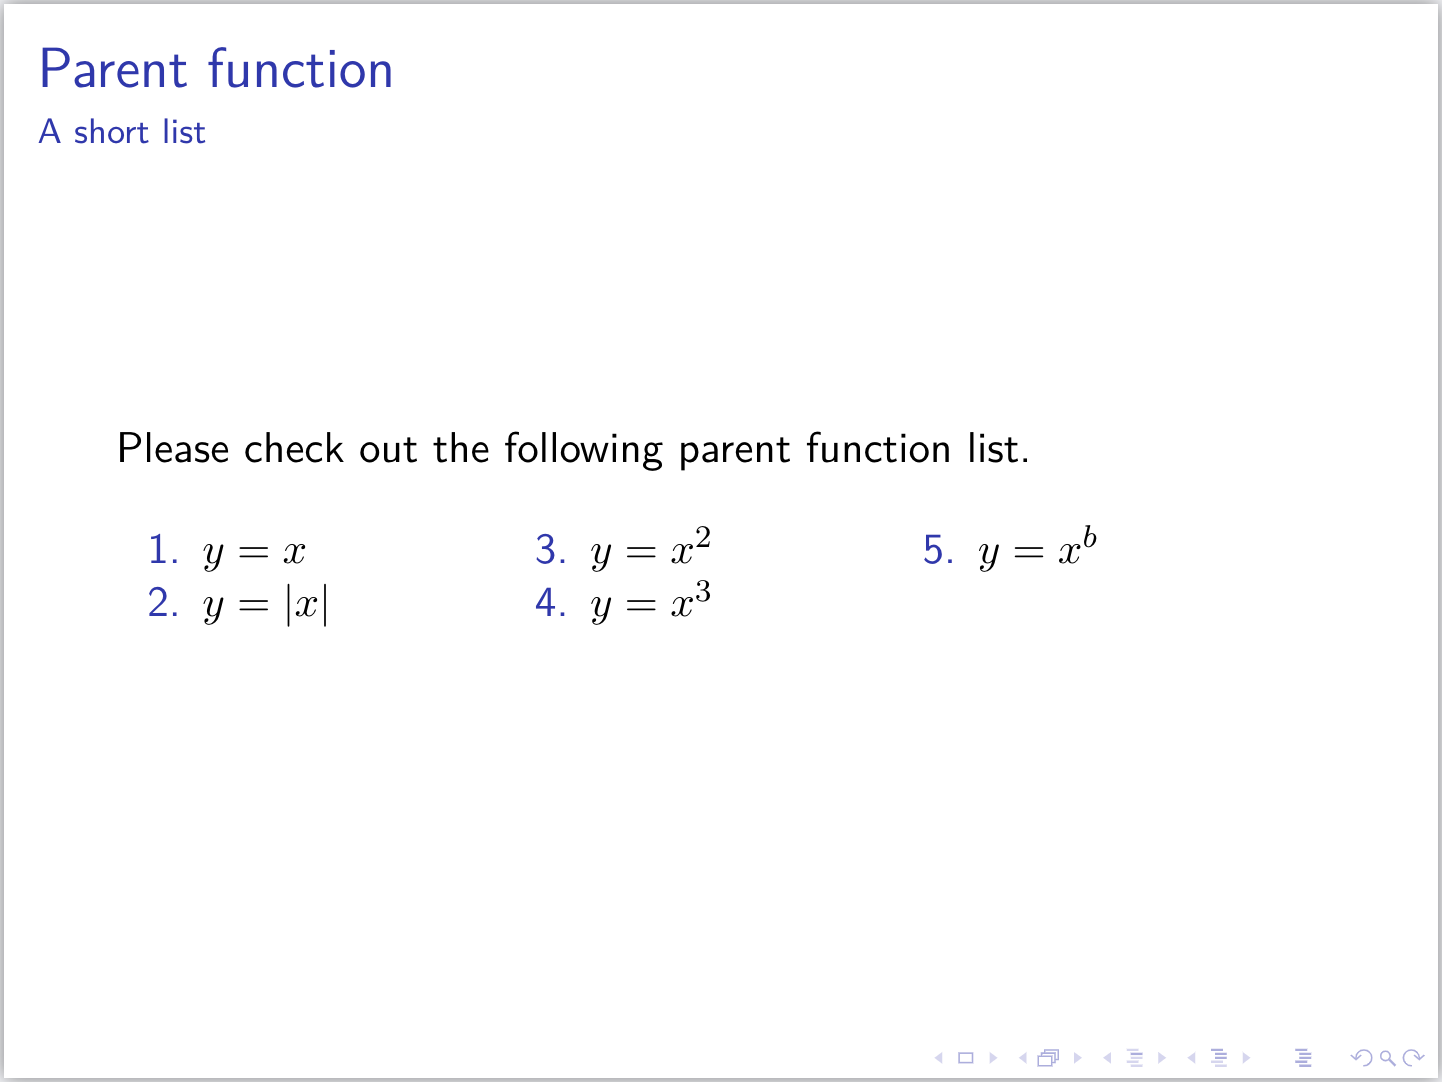
\includegraphics[width = 0.6\linewidth]{images/ch_9/example_multicol.png}
    \caption{编译后的幻灯片效果}
    \label{fig:910}
\end{figure}

\emph{【例】}在beamer文档类型中使用columns环境对幻灯片内容进行分栏处理:
\begin{lstlisting}[language=TeX]
    \documentclass{beamer}
    \usefonttheme{professionalfonts}

    \begin{document}

    \begin{frame}
    \frametitle{Parent function}
    \framesubtitle{A short list}

    \begin{columns}
    \begin{column}{0.5\textwidth}

    Please check out the following parent function list.
    \begin{enumerate}
    \item $y=x$
    \item $y=|x|$
    \item $y=x^{2}$
    \item $y=x^{3}$
    \item $y=x^{b}$
    \end{enumerate}

    \end{column}

    \begin{column}{0.5\textwidth}

    Please check out the following parent function list.
    \begin{enumerate}
    \item $y=x$
    \item $y=|x|$
    \item $y=x^{2}$
    \item $y=x^{3}$
    \item $y=x^{b}$
    \end{enumerate}

    \end{column}
    \end{columns}

    \end{frame}

    \end{document}
\end{lstlisting}

编译后得到的幻灯片如图\ref{fig:911}所示。

\begin{figure}[htbp]
    \centering
    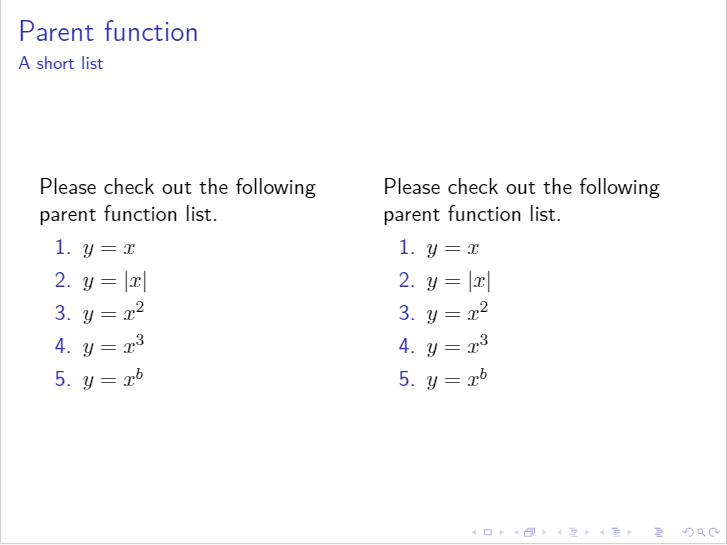
\includegraphics[width = 0.6\linewidth]{images/ch_9/example_two_column.png}
    \caption{编译后的幻灯片效果}
    \label{fig:911}
\end{figure}

\subsubsection{参考资料}
\begin{itemize}
    \item Prathik Naidu, Adam Pahlavan.
          \href{http://web.mit.edu/rsi/www/pdfs/beamer-tutorial.pdf}{Fun with
              Beamer: An Epic Quest To Create the Perfect Presentation}, June 28,
          2017.
\end{itemize}

\section{添加动画效果}

在制作幻灯片时有时需要添加动画效果。由于LaTeX制作幻灯片会被编译成PDF文档,因此,在Beamer中,实现动画效果的方式是将具有动画内容的幻灯片按照次序拆分成若干页内容,在播放时通过翻页达到“动态”视觉效果。为了便于说明,以下将一个frame环境创建的内容称为一页幻灯片或幻灯片页、将动画效果拆分后得到的每一页内容称为该幻灯片的某一帧。

下面介绍在Beamer中常见的几种动画效果命令。

\subsection{pause命令}

\texttt{\textbackslash{}pause}是Beamer中最常用的一种动画效果命令,它的使用方式极其简单,通过在文本或段落中添加\texttt{\textbackslash{}pause}命令,便可将一页幻灯片拆分成若干帧。一般来说,\texttt{\textbackslash{}pause}命令后的内容将会在下一帧中显示,从而使幻灯片在内容显示上呈现出动画效果。比如,一般情况下,使用列表环境创建的每项内容(使用\texttt{\textbackslash{}item}创建)都会在同一帧幻灯片中显示,为了达到各项内容逐个显示的动画效果,可以在两个相邻的\texttt{\textbackslash{}item}语句之间插入\texttt{\textbackslash{}pause}命令。

\emph{【例】}在beamer文档类型中使用pause命令实现一个简单的动画效果:
\begin{lstlisting}[language=TeX]
    \documentclass{beamer}
    \usefonttheme{professionalfonts}

    \begin{document}

    \begin{frame}
    \frametitle{Parent function}
    \framesubtitle{A short list}

    Please check out the following parent function list.
    \begin{enumerate}
    \item $y=x$
    \pause
    \item $y=|x|$
    \pause
    \item $y=x^{2}$
    \pause
    \item $y=x^{3}$
    \pause
    \item $y=x^{b}$
    \end{enumerate}
    \end{frame}

    \end{document}
\end{lstlisting}

编译后得到的幻灯片如图\ref{fig:912}所示。

\begin{figure}[htbp]
    \centering
    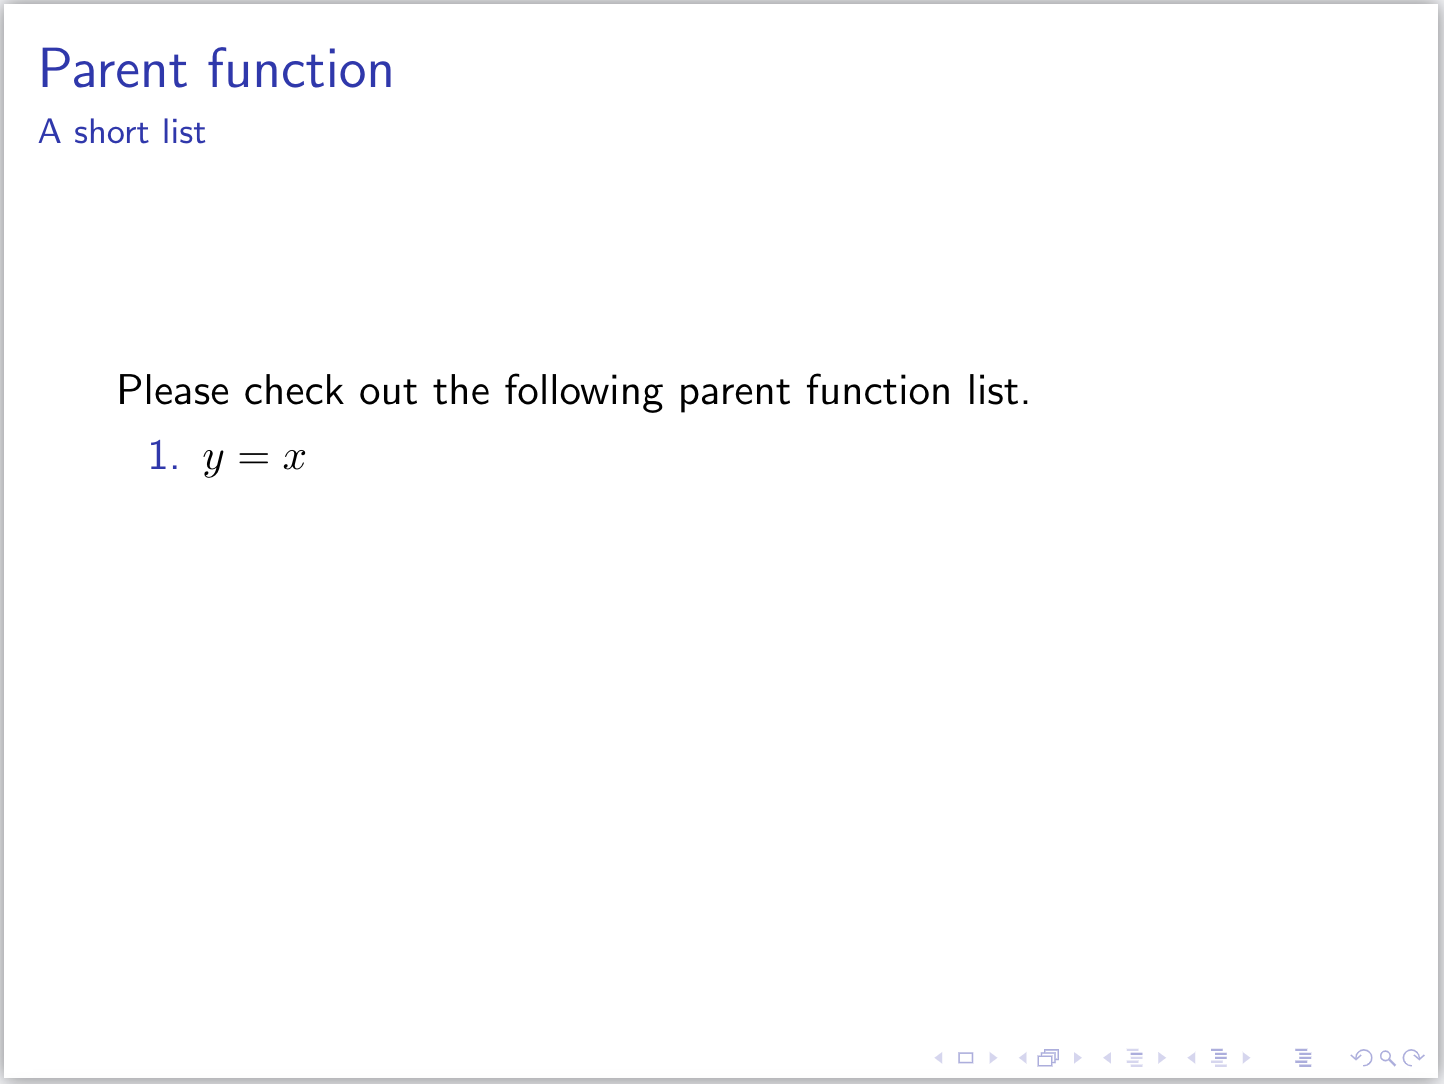
\includegraphics[width = 0.45\linewidth]{images/ch_9/example6_1.png}
    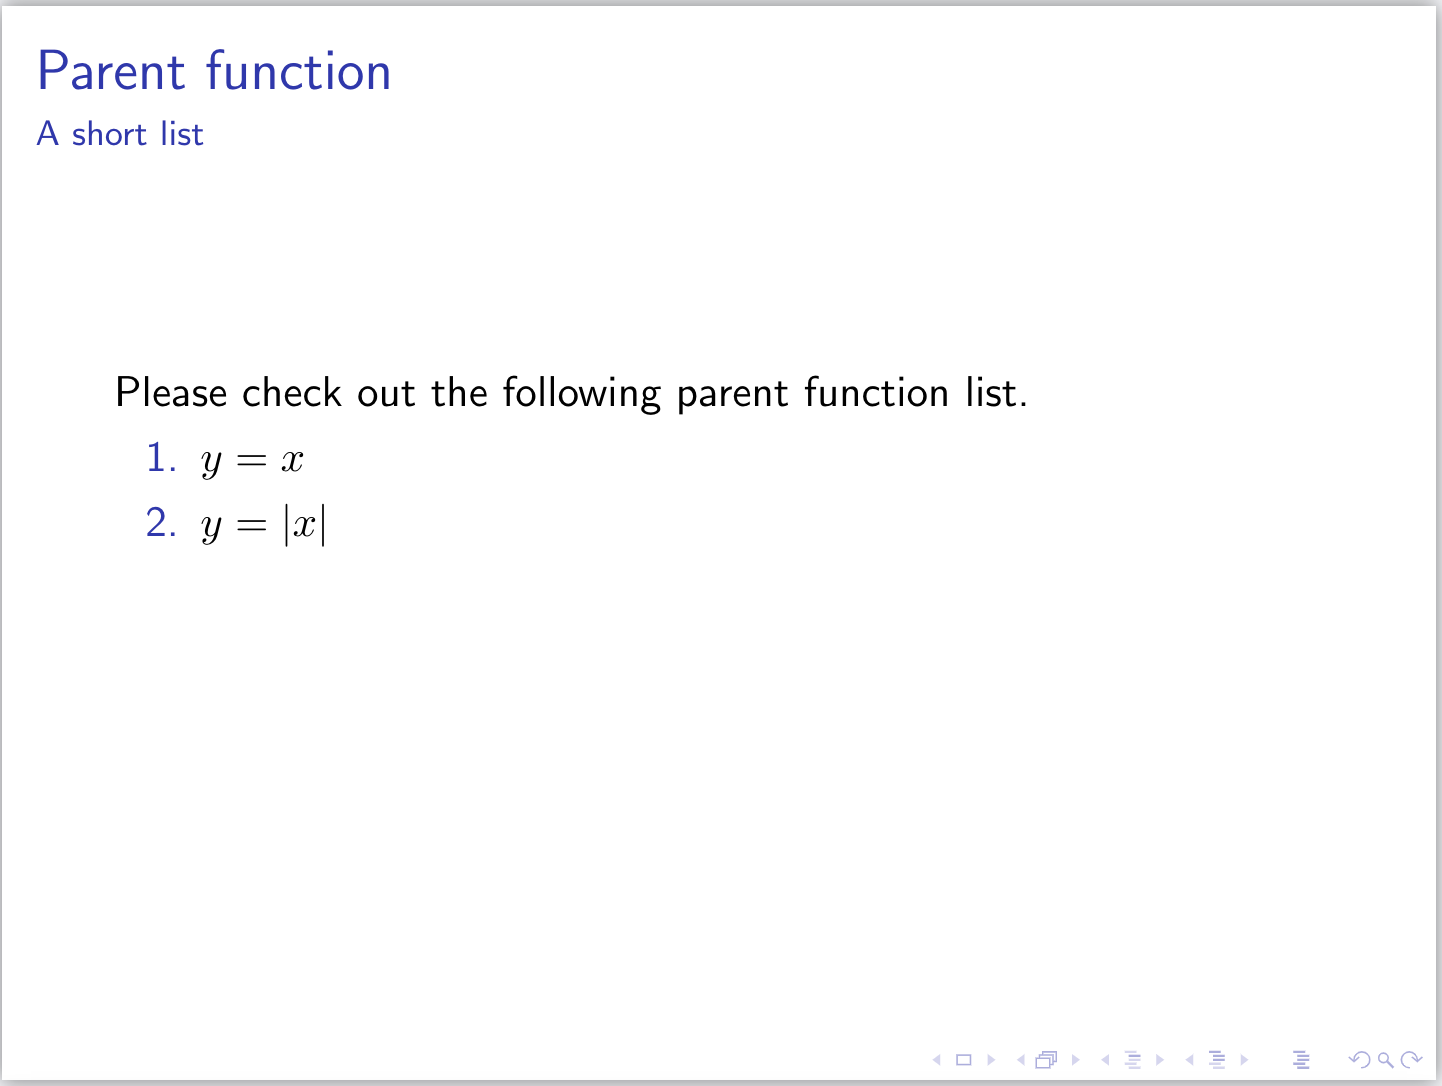
\includegraphics[width = 0.45\linewidth]{images/ch_9/example6_2.png}
    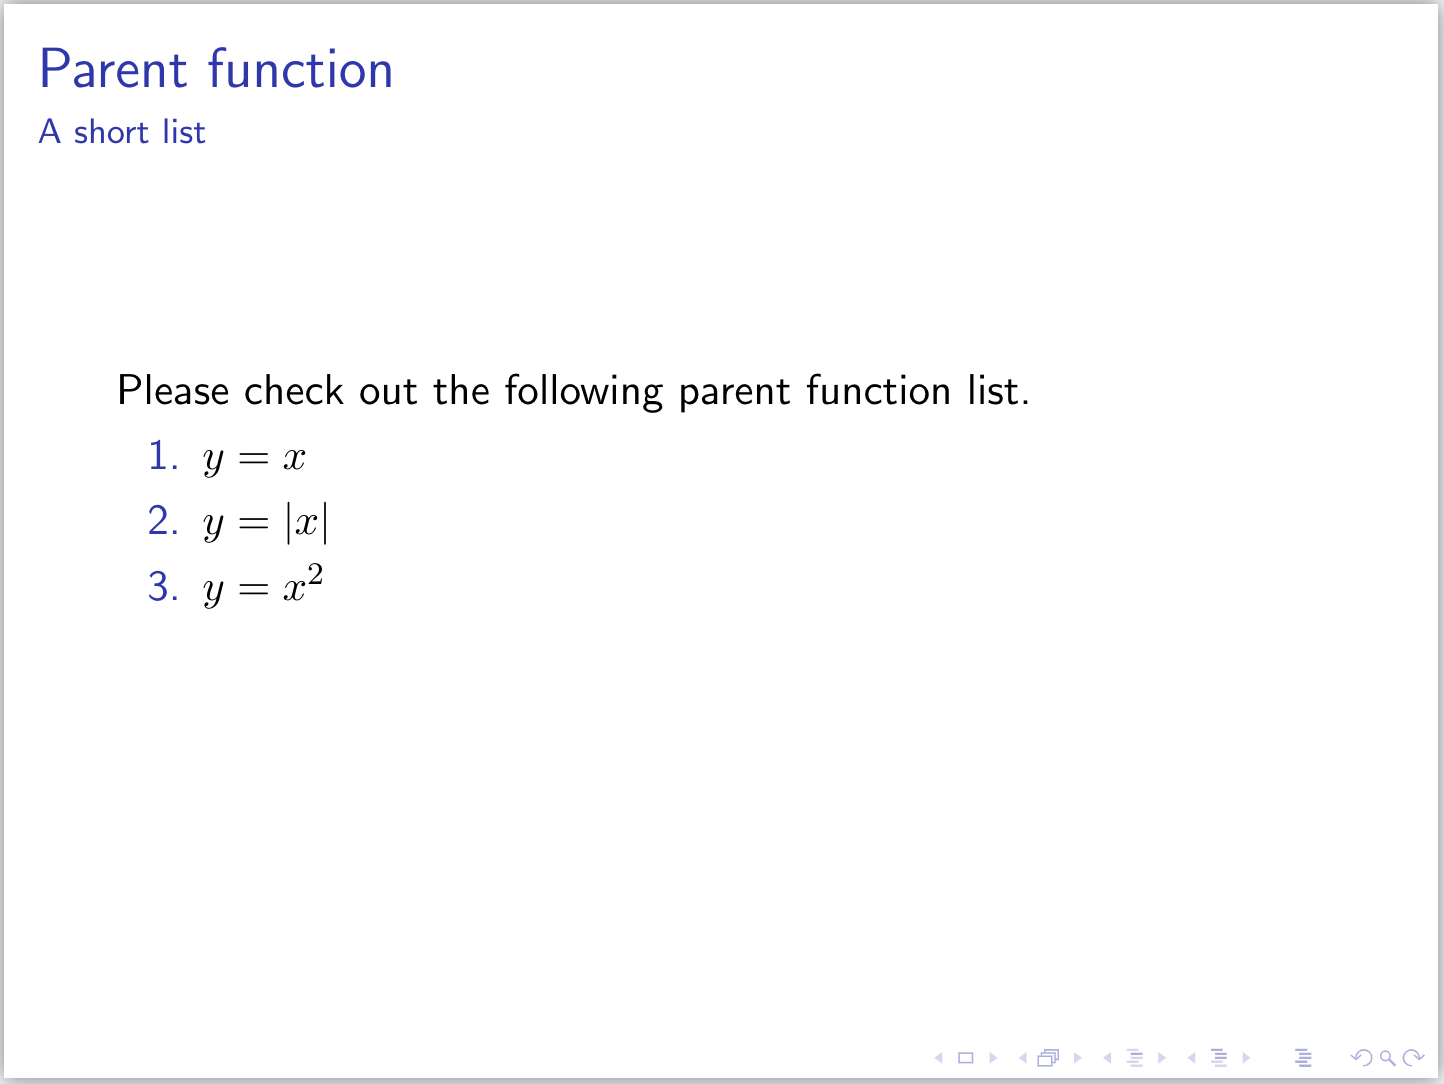
\includegraphics[width = 0.45\linewidth]{images/ch_9/example6_3.png}
    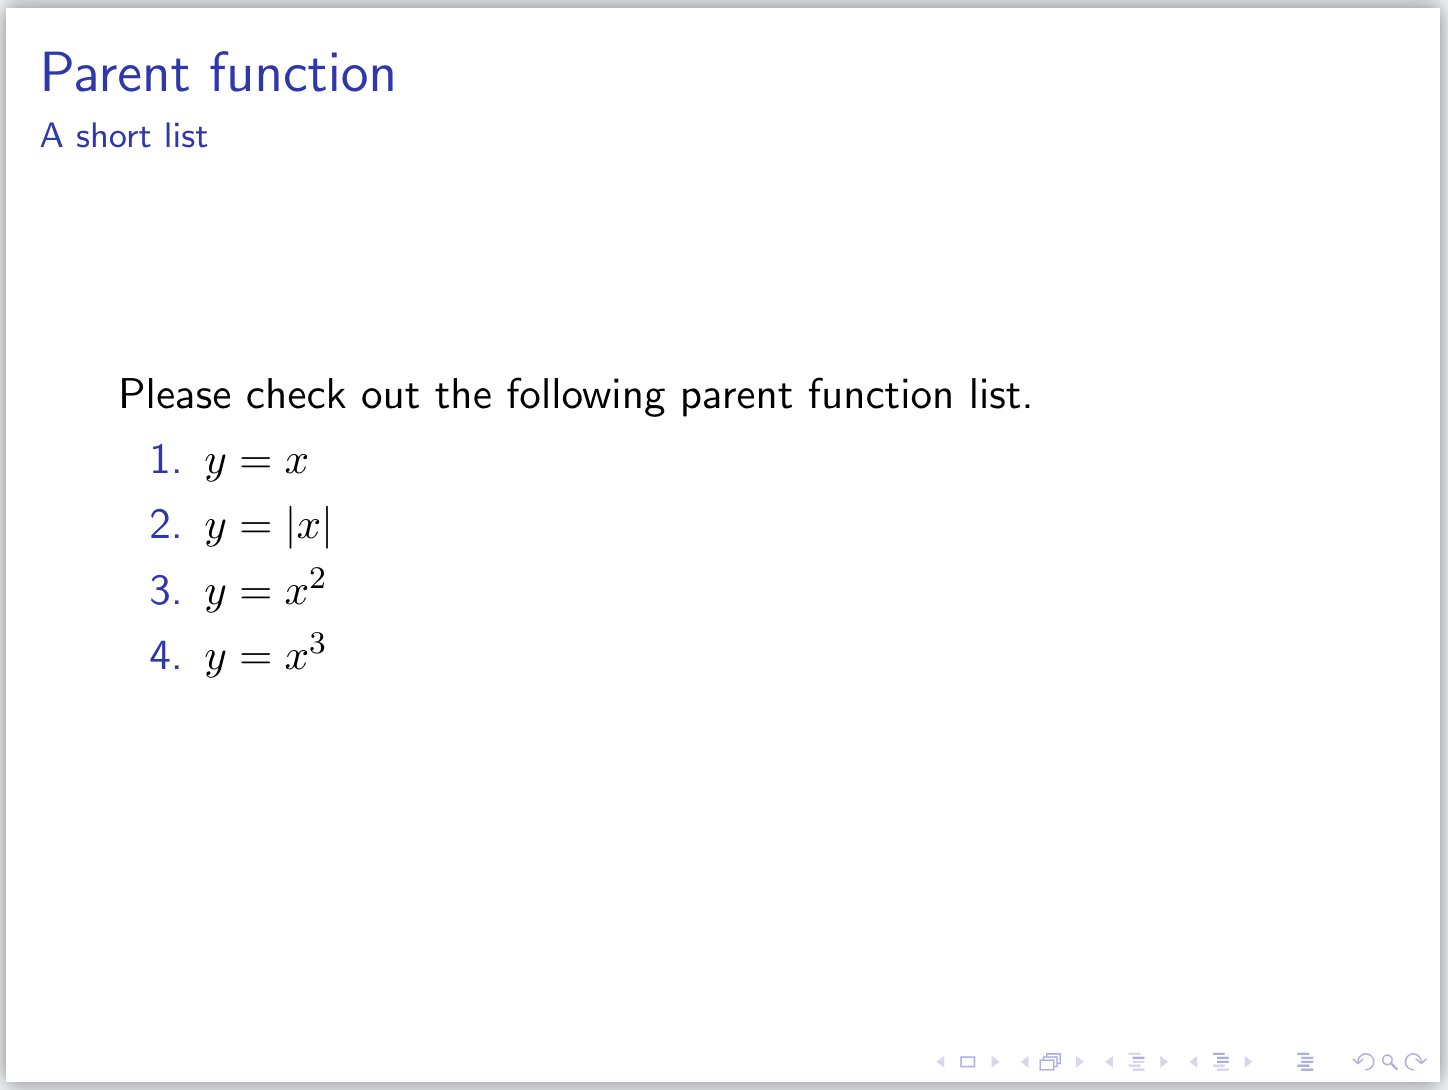
\includegraphics[width = 0.45\linewidth]{images/ch_9/example6_4.png}
    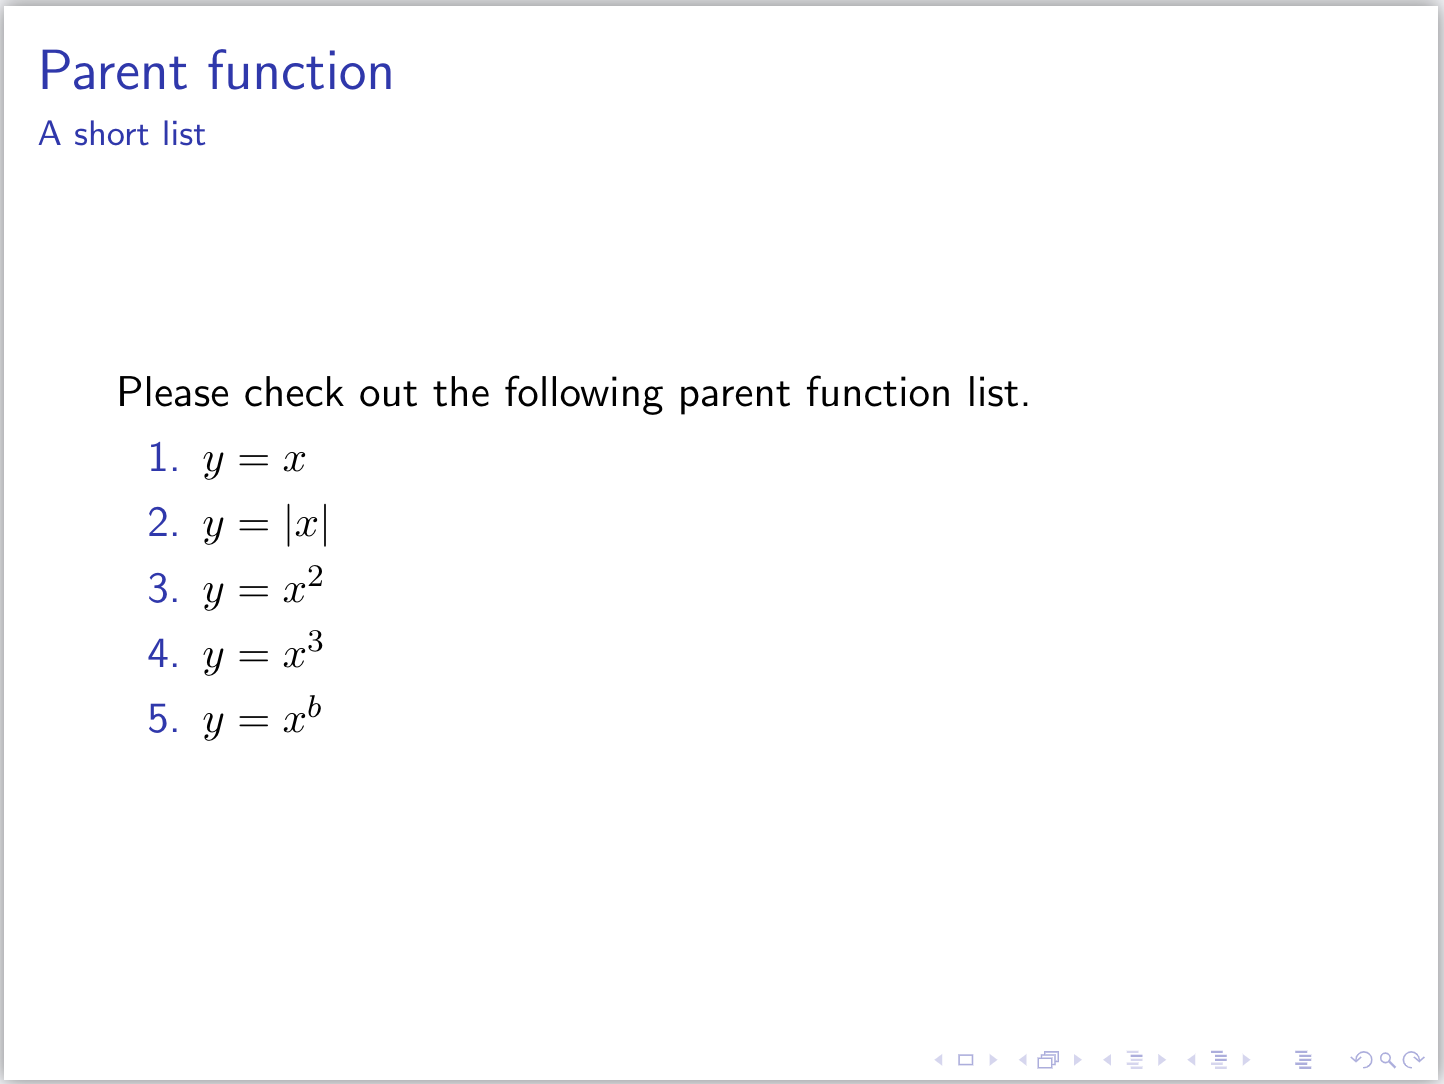
\includegraphics[width = 0.45\linewidth]{images/ch_9/example6_5.png}
    \caption{编译后的幻灯片效果}
    \label{fig:912}
\end{figure}

\subsection{item<>命令}

对于列表环境中的各项内容,也可以通过设置选项指定在该幻灯片的哪些步骤中显示该项内容,从而更加灵活地定制动画效果。具体是使用\texttt{\textbackslash{}item<>},其中<>用于指定显示步骤,对于没有指定<>显示范围的内容项默认会在所有幻灯片页面中显示。具体而言,<>中的内容存在以下四种格式:
\begin{itemize}
    \item <A,B,C>:表示内容项将在第A、B、C步中显示。如,\texttt{\textbackslash{}item<2, 3, 4> \$y=x\^\{2\}\$}表示该项内容将出现在该页幻灯片放映的第2、3、4步;
    \item <A-B>:表示内容项将在第A至B步中显示。如,\texttt{\textbackslash{}item<1-4> \$y=x\$}表示该项内容将出现在该页幻灯片放映的第1~4步;
    \item <A->:表示内容项将在第A步及以后显示。如,\texttt{\textbackslash{}item<2-> \$y=x\$}表示该项内容将出现在该页幻灯片放映的第2步及之后的步骤中;
    \item <-A>:表示内容项将在第A步及之前显示。如,\texttt{\textbackslash{}item<-3> \$y=x\$}表示该项内容将出现在该页幻灯片放映的第3步及之前的步骤中。
\end{itemize}

由此创建的一张幻灯片将包含多帧,其帧数由所有\texttt{\textbackslash{}item<>}命令中设置的最大步骤决定。

如果想要在某一帧中突出某项内容,主要包括以下两种方式:
\begin{itemize}
    \item 使用\texttt{\textbackslash{}alert}命令为该项内容指定需要高亮显示的步骤。具体用法如:\texttt{\textbackslash{}item<2-| alert@3-4> The second item.},此时内容项“The second item.”将出现在第2步之后的步骤中,并通过命令\texttt{\textbackslash{}alert}及前缀@使其在第3~4步中高亮显示。
    \item 使用\texttt{\textbackslash{}color<范围>\{显示颜色\}}命令改变内容项的颜色。如\texttt{\textbackslash{}item<1-> \textbackslash{}color<1>\{red\} The first item.}语句,内容The first item.将出现在第一步及之后的步骤中,通过\texttt{\textbackslash{}color<1>\{red\}}令该项内容在第一步显示颜色为红色,而在其它步骤中仍为默认颜色。
\end{itemize}

\emph{【例】}在beamer文档类型中使用item定制内容显示范围并使用alert对内容项进行高亮显示,从而实现一个简单的动画效果:
\begin{lstlisting}[language=TeX]
    \documentclass{beamer}
    \usefonttheme{professionalfonts}

    \begin{document}

    \begin{frame}
    \frametitle{Parent function}
    \framesubtitle{A short list}

    Please check out the following parent function list.
    \begin{enumerate}
    \item<1-| alert@1> $y=x$
    \item<2-| alert@2> $y=|x|$
    \item<3-| alert@3> $y=x^{2}$
    \item<4-| alert@4> $y=x^{3}$
    \end{enumerate}

    \end{frame}

    \end{document}
\end{lstlisting}

编译后得到的幻灯片如图\ref{fig:913}所示。

\begin{figure}[htbp]
    \centering
    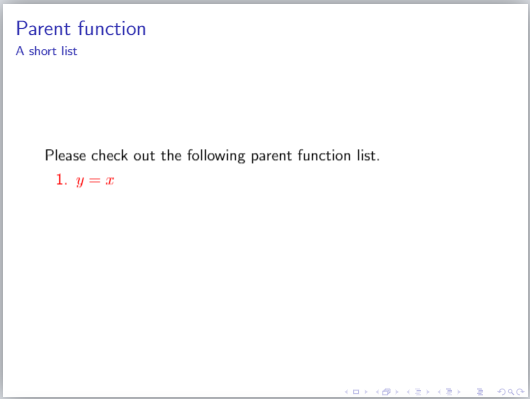
\includegraphics[width = 0.45\linewidth]{images/ch_9/NEWexample7_1.png}
    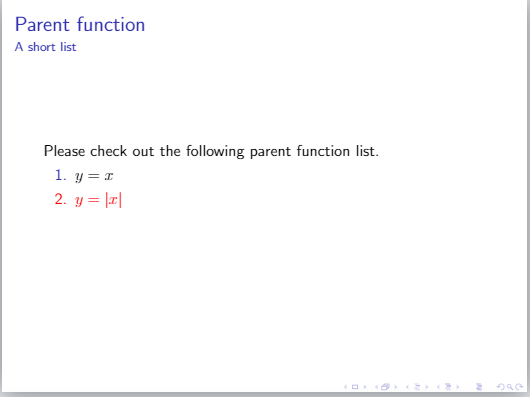
\includegraphics[width = 0.45\linewidth]{images/ch_9/NEWexample7_2.png}
    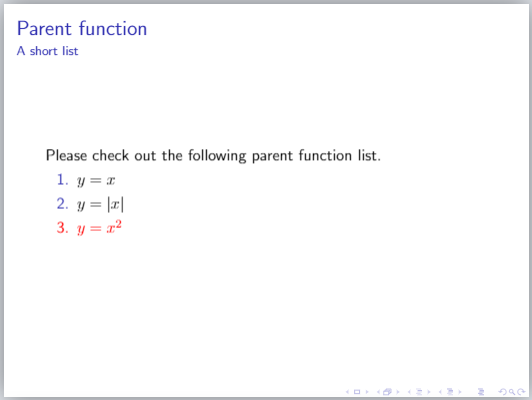
\includegraphics[width = 0.45\linewidth]{images/ch_9/NEWexample7_3.png}
    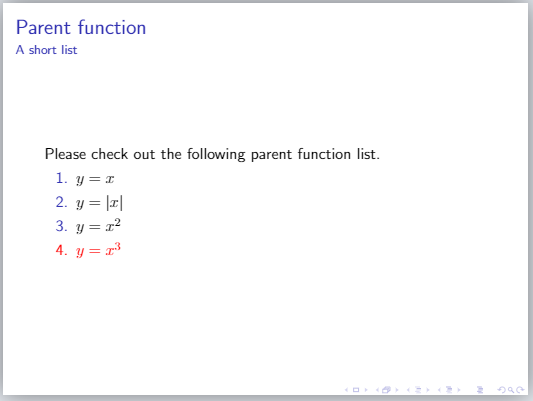
\includegraphics[width = 0.45\linewidth]{images/ch_9/NEWexample7_4.png}
    \caption{编译后的幻灯片效果}
    \label{fig:913}
\end{figure}

\emph{【例】}在beamer文档类型中使用item定制内容显示范围并使用color对内容项进行高亮显示:
\begin{lstlisting}[language=TeX]
    \documentclass{beamer}
    \usefonttheme{professionalfonts}

    \begin{document}

    \begin{frame}
    \frametitle{Parent function}
    \framesubtitle{A short list}

    Please check out the following parent function list.
    \begin{enumerate}
    \item<1-> \color<1>{red} $y=x$
    \item<2-> \color<2>{red} $y=|x|$
    \item<3-> \color<3>{red} $y=x^{2}$
    \item<4-> \color<4>{red} $y=x^{3}$
    \end{enumerate}

    \end{frame}

    \end{document}
\end{lstlisting}

\subsection{其它命令}
LaTeX还提供了其它命令可以实现类似的动画效果,同样可以在可选参数<>中指定内容项或内容块的显示范围,主要包括\texttt{\textbackslash{}onslide}、\texttt{\textbackslash{}uncover}、\texttt{\textbackslash{}only}、\texttt{\textbackslash{}visible}、\texttt{\textbackslash{}invisible}等命令:
\begin{itemize}
    \item \texttt{\textbackslash{}onslide<>\{\}}:该命令可以指定内容在当前幻灯片页放映的第几步显示。使用该命令时不显示的内容将被“遮挡”,仍将占用其指定的位置(\texttt{\textbackslash{}uncover<>\{\}}或\texttt{\textbackslash{}visible<>\{\}}也能实现类似效果);
          \emph{【例】}在beamer文档类型中使用onslide命令实现一个简单的动画效果:
          \begin{lstlisting}[language=TeX]
        \documentclass{beamer}
        \usefonttheme{professionalfonts}

        \begin{document}

        \begin{frame}
        \frametitle{Parent function}
        \framesubtitle{A short list}

        \onslide<1->{Please check out the following parent function list.}

        \onslide<2,4>{1. $y=x$}

        \onslide<1-4>{2. $y=|x|$}

        \onslide<2->{3. $y=x^{2}$}

        \onslide<3->{4. $y=x^{3}$}

        \onslide<4>{5. $y=x^{b}$}

        \end{frame}

        \end{document}
    \end{lstlisting}
    \item \texttt{\textbackslash{}only<>\{\}}:该命令可以指定内容在当前幻灯片页放映的第几步插入。使用该命令时,不显示的内容对应的位置将腾空出来,可以用于显示其它内容;
          \emph{【例】}在beamer文档类型中使用only命令实现一个简单的动画效果:
          \begin{lstlisting}[language=TeX]
        \documentclass{beamer}
        \usefonttheme{professionalfonts}

        \begin{document}

        \begin{frame}
        \frametitle{Parent function}
        \framesubtitle{A short list}

        \only<1->{Please check out the following parent function list.}

        \only<2,4>{1. $y=x$}

        \only<1-4>{2. $y=|x|$}

        \only<2->{3. $y=x^{2}$}

        \only<3->{4. $y=x^{3}$}

        \only<4>{5. $y=x^{b}$}

        \end{frame}

        \end{document}
    \end{lstlisting}

          编译后得到的幻灯片如图\ref{fig:914}所示。

          \begin{figure}[htbp]
              \centering
              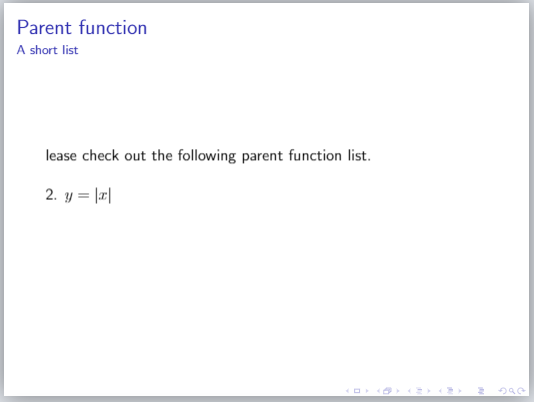
\includegraphics[width = 0.45\linewidth]{images/ch_9/NEWexample2_1.png}
              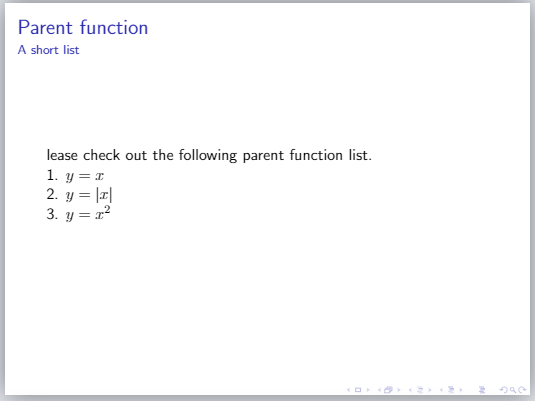
\includegraphics[width = 0.45\linewidth]{images/ch_9/NEWexample2_2.png}
              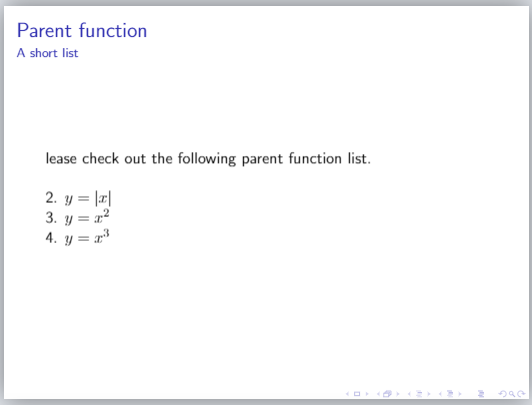
\includegraphics[width = 0.45\linewidth]{images/ch_9/NEWexample2_3.png}
              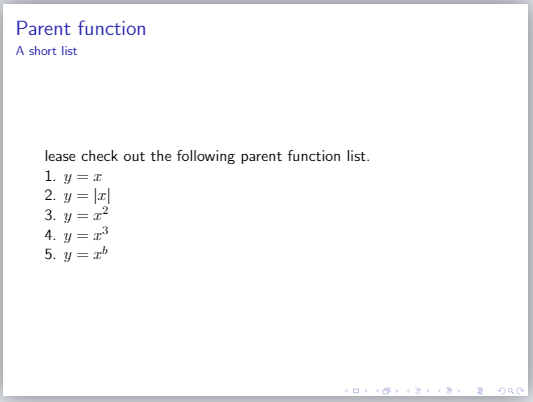
\includegraphics[width = 0.45\linewidth]{images/ch_9/NEWexample2_4.png}
              \caption{编译后的幻灯片效果}
              \label{fig:914}
          \end{figure}

    \item \texttt{\textbackslash{}invisible<>\{\}}:该命令的作用效果与\texttt{\textbackslash{}visible<>\{\}}相反,用于指定内容在当前幻灯片页放映的第几步不可见。但与\texttt{\textbackslash{}visible<>\{\}}相同的是,使用\texttt{\textbackslash{}invisible<>\{\}}命令时,不可见的内容仍占据着对应的位置,不可用于显示其它内容。
          \emph{【例】}在beamer文档类型中使用invisible命令实现一个简单的动画效果:
          \begin{lstlisting}[language=TeX]
        \documentclass{beamer}
        \usefonttheme{professionalfonts}

        \begin{document}

        \begin{frame}
        \frametitle{Parent function}
        \framesubtitle{A short list}

        \visible<1-4>{Please check out the following parent function list.}

        \invisible<1,3>{1. $y=x$}

        \invisible<>{2. $y=|x|$}

        \invisible<1>{3. $y=x^{2}$}

        \invisible<1-2>{4. $y=x^{3}$}

        \invisible<1-3>{5. $y=x^{b}$}

        \end{frame}

        \end{document}
    \end{lstlisting}

          编译后得到的幻灯片如图\ref{fig:915}所示。

          \begin{figure}[htbp]
              \centering
              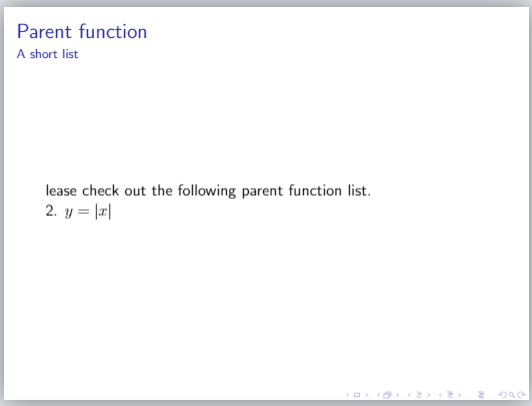
\includegraphics[width = 0.45\linewidth]{images/ch_9/NEWexample3_1.png}
              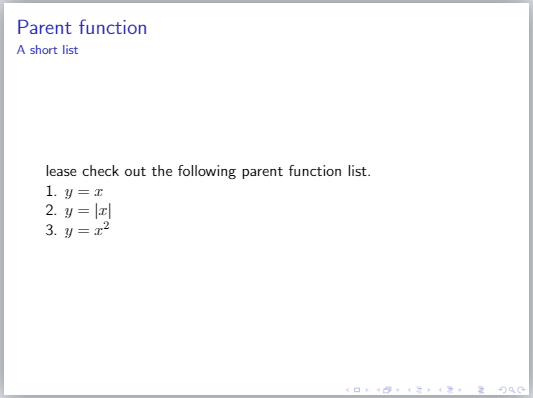
\includegraphics[width = 0.45\linewidth]{images/ch_9/NEWexample3_2.png}
              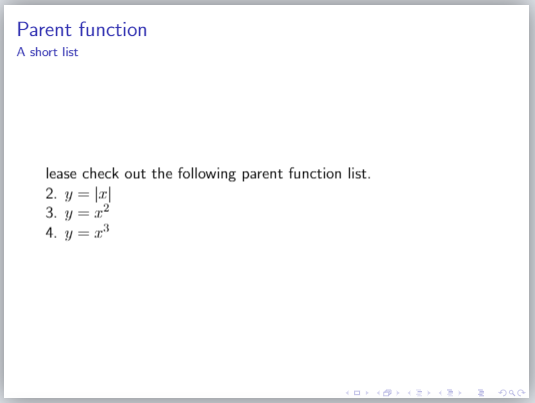
\includegraphics[width = 0.45\linewidth]{images/ch_9/NEWexample3_3.png}
              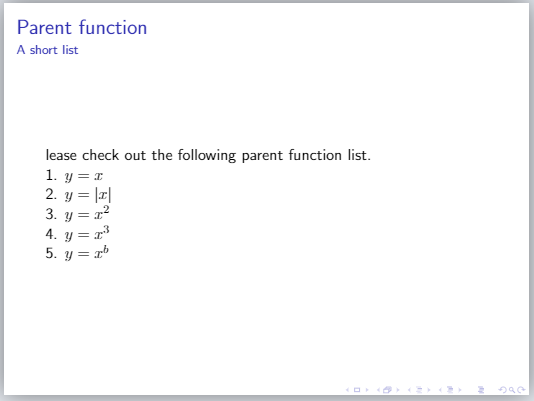
\includegraphics[width = 0.45\linewidth]{images/ch_9/NEWexample3_4.png}
              \caption{编译后的幻灯片效果}
              \label{fig:915}
          \end{figure}
\end{itemize}

\subsection{自动计数}

上述介绍的动画效果定制命令均通过在<>中指定具体的数字指定内容显示范围。此时,如果想要在开始处或中间插入新的内容项,则其余所有内容项的<>显示范围都必须作出相应调整,显然不够灵活。LaTeX提供了一种更巧妙的方式可以解决这类问题:使用“+”号代替具体数字,从1开始进行自动递增计数。就例9-13而言,可以用“+”符号代替各<>中的具体数字,可以得到完全相同的编译效果。修改后的语句如下:
\emph{【例】}在beamer文档类型中使用+符号灵活定制幻灯片效果:
\begin{lstlisting}[language=TeX]
    \documentclass{beamer}
    \usefonttheme{professionalfonts}

    \begin{document}

    \begin{frame}
    \frametitle{Parent function}
    \framesubtitle{A short list}

    Please check out the following parent function list.
    \begin{enumerate}
    \item<+-| alert@+> $y=x$  % 此时“+”号对应数字1
    \item<+-| alert@+> $y=|x|$  % 此时“+”号对应数字2
    \item<+-| alert@+> $y=x^{2}$  % 此时“+”号对应数字3
    \item<+-| alert@+> $y=x^{3}$  % 此时“+”号对应数字4
    \end{enumerate}

    \end{frame}

    \end{document}
\end{lstlisting}

上述语句每一条\texttt{\textbackslash{}item}格式相同,因此也可以简写为如下语句:
\begin{lstlisting}[language=TeX]
    \documentclass{beamer}
    \usefonttheme{professionalfonts}

    \begin{document}

    \begin{frame}
    \frametitle{Parent function}
    \framesubtitle{A short list}

    Please check out the following parent function list.
    \begin{enumerate}[<+-| alert@+>]
    \item $y=x$
    \item $y=|x|$
    \item $y=x^{2}$
    \item $y=x^{3}$
    \end{enumerate}

    \end{frame}

    \end{document}
\end{lstlisting}

有时在<>中使用的数字不总是从1开始递增,那么就需要使用“+(偏移量)”的命令格式。比如,如果当前“+”号对应的计数器值为3,那么<+(2)->意味着在当前计数器值的基础上加2,<+(-2)->则意味着在当前计数器值的基础上减2。

\emph{【例】}在beamer文档类型中使用+(偏移量)符号灵活定制任意显示步骤的幻灯片效果:
\begin{lstlisting}[language=TeX]
    \documentclass{beamer}
    \usefonttheme{professionalfonts}

    \begin{document}

    \begin{frame}
    \frametitle{Parent function}
    \framesubtitle{A short list}

    Please check out the following parent function list.
    \begin{enumerate}
    \item<+(1)-> $y=x$  % 相当于`\item<2-> $y=x$`
    \item<-+(2)> $y=|x|$  % 相当于`\item<-4> $y=|x|$`
    \item<+(-1)-+(1)> $y=x^{2}$  % 相当于`\item<2-4> $y=x^{2}$`
    \item<+(-1)> $y=x^{3}$  % 相当于`\item<3> $y=x^{3}$`
    \end{enumerate}

    \end{frame}

    \end{document}
\end{lstlisting}

编译后得到的幻灯片如图\ref{fig:916}所示。

\begin{figure}[htbp]
    \centering
    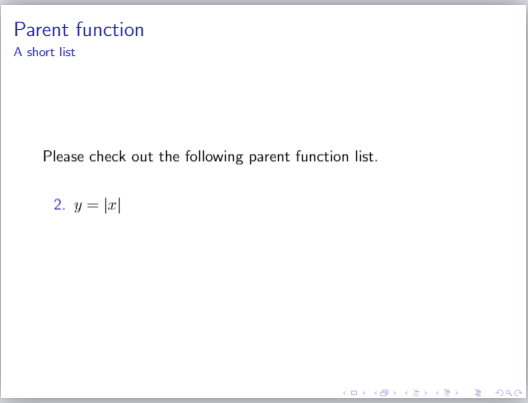
\includegraphics[width = 0.45\linewidth]{images/ch_9/NEWexample10_1.png}
    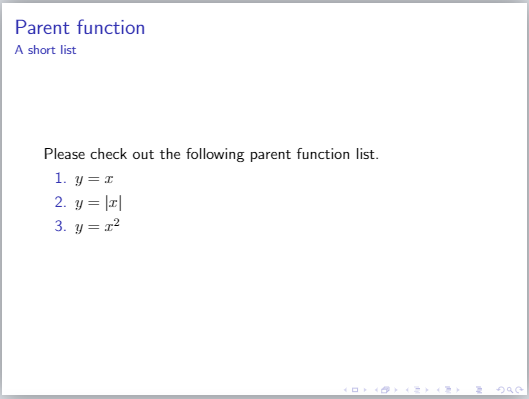
\includegraphics[width = 0.45\linewidth]{images/ch_9/NEWexample10_2.png}
    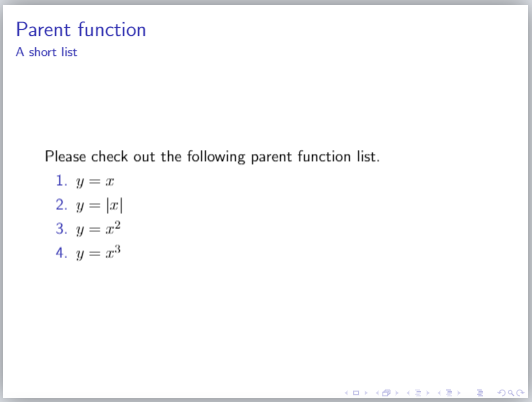
\includegraphics[width = 0.45\linewidth]{images/ch_9/NEWexample10_3.png}
    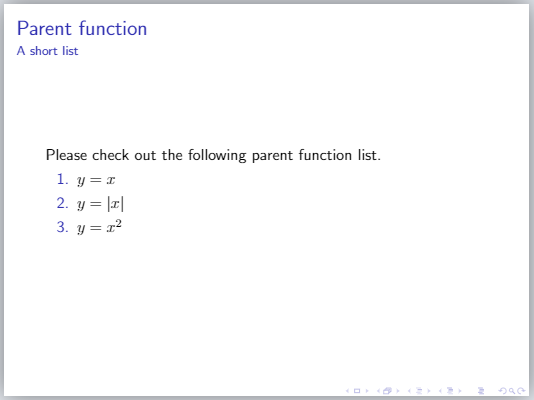
\includegraphics[width = 0.45\linewidth]{images/ch_9/NEWexample10_4.png}
    \caption{编译后的幻灯片效果}
    \label{fig:916}
\end{figure}

\section{块与盒子——添加框元素}

在幻灯片中框选文本或图片等元素是常见的操作,可以对幻灯片内容进行划分或者突出重点内容。在Beamer中,可以通过添加区块环境(block environments)或创建盒子(box)结构的方式将文本等元素放在各式各样的框中。

\subsection{区块环境}

Beamer提供了区块环境(block)可用于编辑文本内容,通过block环境创建的文本内容将放置在一个框中,使其与普通文本区分开。根据内容样式和使用目的的不同,包括三种区块环境:
\begin{itemize}
    \item block:一般性区块环境。使用语法为\texttt{\textbackslash{}begin\{block\}<指定显示步骤>\{设置标题\}} \texttt{\textbackslash{}end\{block\}};
    \item alertblock:警示性区块环境,主要用于创建警示信息。使用语法为\texttt{\textbackslash{}begin\{alertblock\}<指定显示步骤>\{设置标题\}}  \texttt{\textbackslash{}end\{alertblock\}};
    \item exampleblock:示例性区块环境,主要用于创建示例文本。使用语法为\texttt{\textbackslash{}begin\{exampleblock\}<指定显示步骤>\{设置标题\}} \texttt{\textbackslash{}end\{exampleblock\}}。
\end{itemize}

在三种区块环境的开始命令中(如:\texttt{\textbackslash{}begin\{block\}<指定显示步骤>\{设置标题\}},“<>”可用于指定当前区块内容显示的步骤,实现动画效果;第二个“\{\}”可用于设置该区块内容的标题,标题将显示在区块内容的上面。此外,区块内容的样式由使用的Beamer主题样式决定。

\emph{【例】}在beamer文档类型中使用block环境插入一个一般文本框、使用alertblock环境插入一个警示性文本框、以及使用exampleblock环境插入一个示例性文本框:
\begin{lstlisting}[language=TeX]
    \documentclass{beamer}
    \usefonttheme{professionalfonts}
    \usetheme{Copenhagen}

    \begin{document}

    \begin{frame}
    \begin{block}<1>{Block1}
    This is a generic block.
    \end{block}

    \begin{alertblock}<1>{Block2}
    This is an alert block.
    \end{alertblock}

    \begin{exampleblock}<1>{Block3}
    This is an example block.
    \end{exampleblock}
    \end{frame}

    \end{document}
\end{lstlisting}

\subsection{定理类环境}

对于定理、引理、推论、示例等定理类文本,除了可以考虑使用区块环境创建之外,Beamer也预定义了相应的命令环境可供使用,包括:
\begin{itemize}
    \item definition:定义环境。使用语法为\texttt{\textbackslash{}begin\{definition\}<指定显示步骤>\{设置名称\}} \texttt{\textbackslash{}end\{definition\}};
    \item fact:事实环境。使用语法为\texttt{\textbackslash{}begin\{fact\}<指定显示步骤>\{设置名称\}} \texttt{\textbackslash{}end\{fact\}};
    \item theorem:定理环境。使用语法为\texttt{\textbackslash{}begin\{theorem\}<指定显示步骤>\{设置名称\}} \texttt{\textbackslash{}end\{theorem\}};
    \item lemma:引理环境。使用语法为\texttt{\textbackslash{}begin\{lemma\}<指定显示步骤>\{设置名称\}} \texttt{\textbackslash{}end\{lemma\}};
    \item proof:证明环境。使用语法为\texttt{\textbackslash{}begin\{proof\}<指定显示步骤>\{设置名称\}} \texttt{\textbackslash{}end\{proof\}};
    \item corollary:推论环境。使用语法为\texttt{\textbackslash{}begin\{corollary\}<指定显示步骤>\{设置名称\}} \texttt{\textbackslash{}end\{corollary\}};
    \item example:示例环境等。使用语法为\texttt{\textbackslash{}begin\{example\}<指定显示步骤>\{设置名称\}} \texttt{\textbackslash{}end\{example\}}。
\end{itemize}

定理类环境的使用与区块环境类似:使用定理类环境可以创建文本框;开始命令中的“<>”可用于指定当前内容显示的步骤,实现动画效果;第二个“\{\}”可用于设置该定理类内容的名称。不同于区块环境的是:定理类内容的标题默认为对应的定理类型,如在definition环境下,标题即为“Definition”,显示在定理类内容的上方;而定理类内容的名称允许用户自行定制,通常位于定理类内容的左侧,以较大的斜体字标示。

\emph{【例】}在beamer文档类型中使用definition环境插入一个定义文本框、使用theorem环境插入一个定理文本框、以及使用example环境插入一个示例文本框:
\begin{lstlisting}[language=TeX]
    \documentclass{beamer}
    \usefonttheme{professionalfonts}
    \usetheme{Copenhagen}

    \begin{document}

    \begin{frame}{Definition, theorem and example}
    \begin{definition}<1>{Definition Demo}
    This is a definition.
    \end{definition}

    \begin{theorem}<1>{Theorem Demo}
    This is a theorem.
    \end{theorem}

    \begin{example}<1>{Example Demo}
    This is an example.
    \end{example}
    \end{frame}

    \end{document}
\end{lstlisting}

\subsection{Beamer中的盒子}

Beamer也支持通过绘制外框的方式为幻灯片的元素(如,文本、图片等)加上外框,或者说创建盒子(box)。常用的语法包括调用\texttt{\textbackslash{}fbox\{\}}命令绘制简单矩形框、或调用fancybox宏包提供的命令(\texttt{\textbackslash{}shadowbox},\texttt{\textbackslash{}doublebox},\texttt{\textbackslash{}ovalbox}和\texttt{\textbackslash{}Ovalbox})创建不同类型的外框。

\subsubsection{使用fbox命令}

使用\texttt{\textbackslash{}fbox\{\}}命令可以创建简单的矩形盒子,调用以下命令可以对盒子参数进行修改:
\begin{itemize}
    \item \texttt{\textbackslash{}setlength\{\textbackslash{}fboxsep\}\{\}}:设置盒子内的元素与其边框之间的距离,默认值为3pt;
    \item \texttt{\textbackslash{}setlength\{\textbackslash{}fboxrule\}\{\}}:设置盒子边框线的粗细,默认值为0.4pt。
\end{itemize}

此外,盒子之间的行间距可以使用\texttt{\textbackslash{}vskip}命令进行修改。

\emph{【例】}在beamer文档类型中使用fbox命令三个文本盒子、使用setlength命令设置不同参数、并使用vskip命令设置行间距:
\begin{lstlisting}[language=TeX]
    \documentclass{beamer}

    \begin{document}

    \begin{frame}
    \setlength{\fboxsep}{3pt}
    \setlength{\fboxrule}{0.4pt}
    \fbox{This is our 1st text box.}
    \vskip 5mm
    \setlength{\fboxsep}{6pt}
    \setlength{\fboxrule}{0.8pt}
    \fbox{This is our 2nd text box.}
    \vskip 5mm
    \setlength{\fboxsep}{9pt}
    \setlength{\fboxrule}{1.2pt}
    \fbox{This is our 3rd text box.}
    \end{frame}

    \end{document}
\end{lstlisting}

对于较短的文本内容,使用\texttt{\textbackslash{}fbox\{\}}命令可以实现较好的效果。但由于在\texttt{\textbackslash{}fbox\{\}}命令中换行符\texttt{\textbackslash{}\textbackslash{}}不起作用,因此如果要对段落文本或长文本创建盒子,需要先将文本内容放置到段落环境中,然后再调用\texttt{\textbackslash{}fbox\{\}}命令。其中,\texttt{\textbackslash{}begin\{minipage\}[外部对齐方式][高度][内部对齐方式]\{宽度\}\{内容\}} \texttt{\textbackslash{}end\{minipage\}}环境和\texttt{\textbackslash{}parbox[外部对齐][高度][内部对齐]\{宽度\}\{内容\}}命令是比较常用的处理段落的语法。

\emph{【例】}在beamer文档类型中使用fbox命令和minipage环境创建段落文本盒子:
\begin{lstlisting}[language=TeX]
    \documentclass{beamer}

    \begin{document}

    \begin{frame}

    \fbox{
    \begin{minipage}[c][1.8cm][t]{5cm}
    {This is our paragraph text box. This is our paragraph text box. This is our paragraph text box. This is our paragraph text box.}
    \end{minipage}}

    \end{frame}

    \end{document}
\end{lstlisting}

类似地,也可以使用\texttt{\textbackslash{}parbox}命令处理段落文本,与minipage环境类似,该命令也能设置外部对齐方式、高度、内部对齐方式、以及宽度参数。用\texttt{\textbackslash{}parbox}命令改写上例代码,编译得到相同的结果,具体语句如下例所示:

\emph{【例】}在beamer文档类型中使用fbox命令和parbox命令创建段落文本盒子:
\begin{lstlisting}[language=TeX]
    \documentclass{beamer}

    \begin{document}

    \begin{frame}

    \fbox{
    \parbox[c][1.8cm][t]{5cm}
    {This is our paragraph text box. This is our paragraph text box. This is our paragraph text box. This is our paragraph text box.}}

    \end{frame}

    \end{document}
\end{lstlisting}

当然,除了为文本内容创建盒子之外,\texttt{\textbackslash{}fbox}命令也能为图片等非文本内容创建盒子。

\emph{【例】}在beamer文档类型中使用figure环境插入三张图片,并使用fbox命令将三种图片装入一个盒子中:
\begin{lstlisting}[language=TeX]
    \documentclass{beamer}

    \begin{document}

    \begin{frame}

    \begin{figure}
    \centering
    \fbox{
    
\includegraphics[width=0.2\linewidth]{redflower.png}
    
\includegraphics[width=0.2\linewidth]{yellowflower.png}
    
\includegraphics[width=0.2\linewidth]{blueflower.png}
    }
    \caption{Here is a figure box.}
    \end{figure}

    \end{frame}

    \end{document}
\end{lstlisting}

\subsubsection{调用fancybox宏包}

在fancybox宏包中,提供了以下四个命令用来创建不同样式的盒子:
\begin{itemize}
    \item \texttt{\textbackslash{}shadowbox\{\}}:创建阴影盒子;
    \item \texttt{\textbackslash{}doublebox\{\}}:创建两重线盒子;
    \item \texttt{\textbackslash{}ovalbox\{\}}:创建细边线椭圆盒子;
    \item \texttt{\textbackslash{}Ovalbox\{\}}:创建粗边线椭圆盒子。
\end{itemize}

\emph{【例】}在beamer文档类型中使用shadowbox,doublebox,ovalbox和Ovalbox命令创建不同样式的盒子:
\begin{lstlisting}[language=TeX]
    \documentclass{beamer}
    \usepackage{fancybox}
    \begin{document}

    \begin{frame}

    \setlength{\fboxsep}{5pt}
    \setlength{\fboxrule}{2pt}

    \shadowbox{This is a shadowbox.}

    \vskip 5mm

    \doublebox{This is a doublebox.}

    \vskip 5mm

    \ovalbox{This is an ovalbox.}

    \vskip 5mm

    \Ovalbox{This is an Ovalbox.}

    \end{frame}

    \end{document}
\end{lstlisting}

类似地,也可以使用上述命令为图片等非文本元素创建不同样式的盒子。

\emph{【例】}在beamer文档类型中使用figure环境插入四张图片,使用shadowbox,doublebox,ovalbox和Ovalbox命令分别为每张图片创建盒子,并使用parbox命令把图片和标题均包含在盒子中:
\begin{lstlisting}[language=TeX]
    \documentclass{beamer}
    \usepackage{fancybox}
    \begin{document}

    \setlength{\fboxsep}{5pt}
    \setlength{\fboxrule}{2pt}

    \begin{frame}
    \begin{figure}
    \centering
    \shadowbox{
    \parbox[c][6cm][t]{5cm}{
    
\includegraphics[width=1\linewidth]{redflower.png}
    \caption{A red flower.}}}
    \end{figure}
    \end{frame}

    \begin{frame}
    \begin{figure}
    \centering
    \doublebox{
    \parbox[c][6cm][t]{5cm}{
    
\includegraphics[width=1\linewidth]{yellowflower.png}
    \caption{A yellow flower.}}}
    \end{figure}
    \end{frame}

    \begin{frame}
    \begin{figure}
    \centering
    \ovalbox{
    \parbox[c][6cm][t]{5cm}{
    \includegraphics[width=1\linewidth]{blueflower.png}
    \caption{A blue flower.}}}
    \end{figure}
    \end{frame}

    \begin{frame}
    \begin{figure}
    \centering
    \Ovalbox{
    \parbox[c][6cm][t]{5cm}{
    \includegraphics[width=1\linewidth]{magentaflower.png}
    \caption{A magenta flower.}}}
    \end{figure}
    \end{frame}

    \end{document}
\end{lstlisting}

\section{设置主题样式}

使用Beamer制作幻灯片的一道特色就是有现成的主题样式可供选择和直接使用,其中,主题样式对于幻灯片的演示效果而言十分重要,简言之,主题样式就是幻灯片的“外观”,改变幻灯片最简单的方式就是变换不同的主题样式。Beamer中提供的每种主题样式都具有良好的可用性和可读性,这也使得Beamer制作出来的幻灯片看起来十分专业,同时,反复使用的难度也不大。

在英文中,主题对应的英文单词为theme。狭义来看,幻灯片主题是指幻灯片的主题样式;但从广义来看,其实幻灯片主题包括了包括主题样式、颜色主题、字体主题、内部主题、外部主题。

\subsection{基本介绍}

使用Beamer制作幻灯片时,我们可以选择很多已经封装好的幻灯片主题样式,不同样式可以达到不同的视觉效果。其实,使用这些主题样式的方法非常简单。通常来说,在前导代码中插入\texttt{\textbackslash{}usetheme\{\}}命令即可,例如使用Copenhagen(哥本哈根主题样式)只需要在前导代码中申明\texttt{\textbackslash{}usetheme\{Copenhagen\}},这种方式调用主题样式是非常省事。

\begin{figure}[htbp]
    \centering
    \includegraphics[width = 0.8\textwidth]{images/ch_9/beamer_theme.pdf}
    \caption{Beamer文档类型中的主题样式}
    \label{figeg:001}
\end{figure}

在Beamer文档类型中,有几十种主题样式可供选择和使用,比较常用的主题样式包括以下这些:
\begin{itemize}
    \item Berlin:柏林主题样式,默认样式为蓝色调;
    \item Copenhagen: 哥本哈根主题样式,默认样式为蓝色调;
    \item CambridgeUS:美国剑桥主题样式,默认样式为红色调;
    \item Berkeley:伯克利主题样式,默认样式为蓝色调;
    \item Singapore:新加坡主题样式;
    \item Warsaw:默认样式为蓝色调。
\end{itemize}

\emph{【例】}在beamer文档类型中使用CambridgeUS主题样式制作一个简单的幻灯片:
\begin{lstlisting}[language=TeX]
    \documentclass{beamer}
    \usetheme{CambridgeUS}
    
    \begin{document}
    
    \begin{frame}{Example}
    
    This is a simple example for the CambridgeUS theme.
    
    \end{frame}
    
    \end{document}
\end{lstlisting}

编译上述代码,得到幻灯片如图\ref{figeg:002}所示。

\begin{figure}[htbp]
    \centering
    \includegraphics[width = 0.8\textwidth]{images/ch_9/example_sec2_1.png}
    \caption{编译后的幻灯片效果}
    \label{figeg:002}
\end{figure}

当然,在这些主题样式基础上,我们也能够使用一些特定的主题样式如颜色主题、字体主题、内部主题、外部主题对幻灯片的显示效果进行调整。

\begin{figure}[htbp]
    \centering
    \includegraphics[width = 0.8\textwidth]{images/ch_9/other_themes.pdf}
    \caption{Beamer文档类型中的其他几种主题设置}
    \label{figeg:003}
\end{figure}

\subsection{颜色主题}

使用Beamer制作幻灯片时,我们能够自行设置幻灯片主题样式的色调,使用\texttt{\textbackslash{}usecolortheme\{\}}命令即可,这些色调包括beetle、beaver、orchid、whale、dolphin等。这里的色调又被称为颜色主题,它定义了幻灯片各部分的颜色搭配,设置特定的颜色主题后,我们能够得到不同的组合样式,具体可参考https://hartwork.org/beamer-theme-matrix/网站提供的组合样式矩阵。

\emph{【例】}在beamer文档类型中使用CambridgeUS主题样式和dolphin色调制作一个简单的幻灯片:
\begin{lstlisting}[language=TeX]
    \documentclass{beamer}
    \usetheme{CambridgeUS}
    \usecolortheme{dolphin}

    \begin{document}

    \begin{frame}{Example}

    This is a simple example for the CambridgeUS theme with dolphin (color theme).

    \end{frame}

    \end{document}
\end{lstlisting}

编译上述代码,得到幻灯片如图\ref{figeg:003}所示。

\begin{figure}[htbp]
    \centering
    \includegraphics[width = 0.8\textwidth]{images/ch_9/example_sec2_2.png}
    \caption{编译后的幻灯片效果}
    \label{figeg:003}
\end{figure}

\subsection{字体主题}

实际上,对于幻灯片的文本字体,我们可以调用字体样式对其进行调整。在Beamer中,字体样式被称为字体主题,它定义了幻灯片的字体搭配。具体使用方法是:在前导代码中要用到的命令为\texttt{\textbackslash{}usefonttheme{A}},位置A填写的一般是字体类型,例如serif。

\emph{【例】}使用beamer文档类型创建一个简单的幻灯片,并在前导代码中申明使用serif对应的字体样式:
\begin{lstlisting}[language=TeX]
    \documentclass{beamer}
    \usefonttheme{serif}

    \begin{document}

    \begin{frame}

    This is a simple example for using \alert{serif} font theme.

    \end{frame}

    \end{document}
\end{lstlisting}

编译上述代码,得到幻灯片如图\ref{figeg:004}所示。

\begin{figure}[htbp]
    \centering
    \includegraphics[width = 0.8\textwidth]{images/ch_9/example_sec2_3.png}
    \caption{编译后的幻灯片效果}
    \label{figeg:004}
\end{figure}

我们知道:在常规文档中,可以使用各种字体对应的宏包达到调用字体的作用,使用规则为\texttt{\textbackslash{}usepackage\{A\}},位置A填写的一般是字体类型,包括serif、avant、bookman、chancery、charter、euler、helvet、mathtime、mathptm、mathptmx、newcent、palatino、pifont、utopia等。

\emph{【例】}使用beamer文档类型创建一个简单的幻灯片,并在前导代码中申明使用字体palatino对应的宏包:
\begin{lstlisting}[language=TeX]
    \documentclass{beamer}
    \usepackage{palatino}

    \begin{document}

    \begin{frame}

    This is a simple example for using \alert{palatino} font.

    \end{frame}

    \end{document}
\end{lstlisting}

编译上述代码,得到幻灯片如图\ref{figeg:005}所示。

\begin{figure}[htbp]
    \centering
    \includegraphics[width = 0.8\textwidth]{images/ch_9/example_sec2_4.png}
    \caption{编译后的幻灯片效果}
    \label{figeg:005}
\end{figure}

\subsection{内部主题}

内部主题定义了幻灯片展示区域的样式,如列表、定理等,内部主题不包括页眉、页脚、导航栏等部分。每一种主题样式都有默认的内部主题,更换内部主题需使用\texttt{\textbackslash{}useinnertheme\{A\}}命令,位置A可供选择的内部主题包括circles、rectangles、rounded和inmargin。

\emph{【例】}在beamer文档类型中分别使用circles内部主题制作幻灯片:
\begin{lstlisting}[language=TeX]
    \documentclass{beamer}
    \usetheme{CambridgeUS}
    \usefonttheme{professionalfonts}
    \useinnertheme{circles}

    \begin{document}

    \begin{frame}
    \frametitle{Parent function}
    \framesubtitle{A short list}

    Please check out the following parent function list.
    \begin{enumerate}
    \item $y=x$
    \item $y=|x|$
    \item $y=x^{2}$
    \item $y=x^{3}$
    \item $y=x^{b}$
    \end{enumerate}

    \end{frame}

    \end{document}
\end{lstlisting}

编译上述代码,得到幻灯片如图\ref{figeg:006}所示。

\begin{figure}[htbp]
    \centering
    \includegraphics[width = 0.8\textwidth]{images/ch_9/example_innertheme_circles.png}
    \caption{编译后的幻灯片效果}
    \label{figeg:006}
\end{figure}

\emph{【例】}在beamer文档类型中分别使用inmargin内部主题制作幻灯片:
\begin{lstlisting}[language=TeX]
    \documentclass{beamer}
    \usetheme{CambridgeUS}
    \usefonttheme{professionalfonts}
    \useinnertheme{inmargin}

    \begin{document}

    \begin{frame}
    \frametitle{Parent function}
    \framesubtitle{A short list}

    Please check out the following parent function list.
    \begin{enumerate}
    \item $y=x$
    \item $y=|x|$
    \item $y=x^{2}$
    \item $y=x^{3}$
    \item $y=x^{b}$
    \end{enumerate}

    \end{frame}

    \end{document}
\end{lstlisting}

编译上述代码,得到幻灯片如图\ref{figeg:007}所示。

\begin{figure}[htbp]
    \centering
    \includegraphics[width = 0.8\textwidth]{images/ch_9/example_innertheme_inmargin.png}
    \caption{编译后的幻灯片效果}
    \label{figeg:007}
\end{figure}

\subsection{外部主题}

外部主题定义了幻灯片的边框、页眉、页脚、导航栏等部分的样式。更换外部主题需使用\texttt{\textbackslash{}useoutertheme\{A\}},位置A可供选择的外部主题包括infolines、smoothbars、sidebar、split和tree。

\subsection{表格字体大小}

在Beamer中制作表格,当我们想对表头或者表格内容文字大小进行调整时,可以使用在前导代码中申明使用\emph{caption}宏包,即\texttt{\textbackslash{}usepackage\{caption\}},然后设置具体的字体大小即可,如\texttt{\textbackslash{}captionsetup\{font = scriptsize, labelfont = scriptsiz\}}可以将表头和表格内容字体大小调整为scriptsize。

\emph{【例】}使用table环境创建一个简单表格,并使用caption宏包将表头字体大小设置为Large、将表格内容字体大小设置为large:
\begin{lstlisting}[language=TeX]
    \documentclass{beamer}
    \usepackage{booktabs}
    \usepackage{caption}
    \captionsetup{font = large, labelfont = Large}

    \begin{document}

    \begin{frame}

    \begin{table}
    \caption{A simple table.}
    \begin{tabular}{l|ccc}
    \toprule
    & \textbf{header3} & \textbf{header4} & \textbf{header5} \\
    \midrule
    \textbf{header1} & cell1 & cell2 & cell3 \\
    \midrule
    \textbf{header2} & cell4 & cell5 & cell6 \\
    \bottomrule
    \end{tabular}
    \end{table}

    \end{frame}

    \end{document}
\end{lstlisting}

编译上述代码,得到幻灯片如图\ref{figeg:008}所示。

\begin{figure}[htbp]
    \centering
    \includegraphics[width = 0.8\textwidth]{images/ch_9/example_sec2_5.png}
    \caption{编译后的幻灯片效果}
    \label{figeg:008}
\end{figure}

其中,单就设置表头字体大小而言,除了使用caption宏包之外,还可以通过对幻灯片设置全局参数达到调整字体大小的效果,例如\texttt{\textbackslash{}setbeamerfont\{caption\}\{size = \textbackslash{}Large\}}。

\subsection{样式调整}

在Beamer文档类型中,除了可以使用各种主题样式,另外也可以根据幻灯片组成部分,分别对侧边栏、导航栏以及Logo等进行调整。其中,侧边栏是由所选幻灯片主题样式自动生成的,主要用于显示幻灯片目录。有时为了显示幻灯片的层次,使用侧边栏进行目录索引。

\emph{【例】}使用Berkeley主题样式,并将侧边栏显示在右侧:
\begin{lstlisting}[language=TeX]
    \documentclass{beamer}
    \PassOptionsToPackage{right}{beamerouterthemesidebar}
    \usetheme{Berkeley}
    \usefonttheme{professionalfonts}

    \begin{document}

    \begin{frame}
    \frametitle{Parent function}
    \framesubtitle{A short list}

    Please check out the following parent function list.
    \begin{enumerate}
    \item $y=x$
    \item $y=|x|$
    \item $y=x^{2}$
    \item $y=x^{3}$
    \item $y=x^{b}$
    \end{enumerate}

    \end{frame}

    \end{document}
\end{lstlisting}

编译上述代码,得到幻灯片如图\ref{figeg:009}所示。

\begin{figure}[htbp]
    \centering
    \includegraphics[width = 0.8\textwidth]{images/ch_9/example_sec2_6.png}
    \caption{编译后的幻灯片效果}
    \label{figeg:009}
\end{figure}

很多时候我们会发现,在各类学术汇报中,幻灯片的首页通常会有主讲人所在的研究机构Logo。在Beamer文档类型中,有\texttt{\textbackslash{}logo}和\texttt{\textbackslash{}titlegraphic}两个命令可供使用,使用\texttt{\textbackslash{}logo}命令添加的Logo会在每一页幻灯片中都显示,而使用\texttt{\textbackslash{}titlegraphic}命令添加的Logo只出现在标题页。

\emph{【例】}使用logo命令在幻灯片中添加Logo:
\begin{lstlisting}[language=TeX]
    \documentclass{beamer}
    \usefonttheme{professionalfonts}

    \title{A Simple Beamer Example}
    \author{Author's Name}
    \institute{Author's Institute}

    \logo{\includegraphics[width=2cm]{logopolito}}

    \begin{document}

    \begin{frame}
    \titlepage
    \end{frame}

    \begin{frame}{Parent function}{A short list}
    Please check out the following parent function list.
    \begin{enumerate}
    \item $y=x$
    \item $y=|x|$
    \item $y=x^{2}$
    \item $y=x^{3}$
    \item $y=x^{b}$
    \end{enumerate}
    \end{frame}

    \end{document}
\end{lstlisting}

编译上述代码,得到幻灯片如图\ref{figeg:010}所示。

\begin{figure}[htbp]
    \centering
    \includegraphics[width = 0.45\textwidth]{images/ch_9/example_sec2_7_0.png}
    \includegraphics[width = 0.45\textwidth]{images/ch_9/example_sec2_7_1.png}
    \caption{编译后的幻灯片效果}
    \label{figeg:010}
\end{figure}

\emph{【例】}使用titlegraphic命令在幻灯片的标题页添加Logo:
\begin{lstlisting}[language=TeX]
    \documentclass{beamer}
    \usefonttheme{professionalfonts}

    \title{A Simple Beamer Example}
    \author{Author's Name}
    \institute{Author's Institute}

    \titlegraphic{\includegraphics[width=2cm]{logopolito}\hspace*{4.75cm}~
    \includegraphics[width=2cm]{logopolito}
    }

    \begin{document}

    \begin{frame}
    \titlepage
    \end{frame}

    \begin{frame}{Parent function}{A short list}
    Please check out the following parent function list.
    \begin{enumerate}
    \item $y=x$
    \item $y=|x|$
    \item $y=x^{2}$
    \item $y=x^{3}$
    \item $y=x^{b}$
    \end{enumerate}
    \end{frame}

    \end{document}
\end{lstlisting}

编译上述代码,得到幻灯片如图\ref{figeg:011}所示。

\begin{figure}[htbp]
    \centering
    \includegraphics[width = 0.45\textwidth]{images/ch_9/example_sec2_8_0.png}
    \includegraphics[width = 0.45\textwidth]{images/ch_9/example_sec2_8_1.png}
    \caption{编译后的幻灯片效果}
    \label{figeg:011}
\end{figure}